\documentclass[a4paper, 11pt, oneside]{report}

\newcommand{\plogo}{\fbox{$\mathcal{PL}$}}
\usepackage{graphicx}
\usepackage{graphics}
\usepackage{float}
\usepackage[table,xcdraw]{xcolor}
\usepackage[utf8]{inputenc}
\usepackage[T1]{fontenc}
\usepackage{fouriernc}
\usepackage{subcaption}
\usepackage{tikz}
\usetikzlibrary{positioning,arrows.meta,shapes.geometric,shapes.multipart,fit,calc,backgrounds}
\usepackage{pgfplots}
\pgfplotsset{compat=1.16}
\usepackage{graphics}
\usepackage{longtable}
\usepackage{array}
\usepackage{tabularx}
\usepackage{listings}
\usepackage[nottoc]{tocbibind}
\usepackage{url}
\usepackage{hyperref}
\usepackage{amsmath}
\usepackage{lipsum}

% ---------- table column types (all tables fit exactly in \textwidth) ----------
\newcolumntype{L}[1]{>{\raggedright\arraybackslash}p{#1}}
\newcolumntype{C}[1]{>{\centering\arraybackslash}p{#1}}
\newcolumntype{Y}{>{\raggedright\arraybackslash}X}
\renewcommand{\arraystretch}{1.3}
\newcommand{\headrow}{\rowcolor{gray!15}}

% ---------- contents: chapters and sections only (keeps it to two pages) ----------
\setcounter{tocdepth}{1}

\lstset{
  basicstyle=\ttfamily\footnotesize,
  breaklines=true,
  frame=single,
  columns=fullflexible,
  keepspaces=true,
  showstringspaces=false,
  numbers=left,
  numberstyle=\tiny,
  xleftmargin=2em
}

\begin{document}
	\begin{titlepage}

		\centering

		\vspace*{\baselineskip}

		\vspace{0.75\baselineskip}

		{\LARGE AI-Powered Team Meeting Assistant\\[0.3\baselineskip]
		\large A Local Multi-Agent System for Structured Software Project Discussions}

		\vspace{0.75\baselineskip}

		\vspace{2\baselineskip}

		A report submitted for the course named Project - II (CS4202)

		\vspace*{5\baselineskip}

		Submitted By

		\vspace{0.5\baselineskip}

		{\scshape\Large Shreya Goswami \\ SEMESTER - VII \\ 230101009}

		\vspace{0.5\baselineskip}

		Supervised By

		\vspace{0.5\baselineskip}

		{\scshape\Large Dr. Sunita Warjri}

		\vspace{0.5\baselineskip}

		\vfill

		\begin{center}
			
\includegraphics[width=5cm]{report_file/iiit manipur.png}
		\end{center}

	{\scshape\small Department of Computer Science and Engineering\\ Indian Institute of Information Technology Senapati, Manipur \\ November, 2026}

\end{titlepage}

%----------------------------------------------------------------------------------------
% Declaration
\begin{center}
   { \LARGE \textbf{Declaration}}
\end{center}
In this submission, I have expressed my idea in my own words, and I have adequately cited and referenced any ideas or words that were taken from another source. I also declare that I adhere to all principles of academic honesty and integrity and that I have not misrepresented or falsified any ideas, data, facts, or sources in this submission. If any violation of the above is made, I understand that the institute may take disciplinary action. Such a violation may also engender disciplinary action from the sources which were not properly cited or permission not taken when needed.

\vspace{1cm}\hspace{8.35cm} Shreya Goswami \\
\vspace{1cm}\hspace{9cm} 230101009 \\
\vspace{1CM} DATE: 05-11-2026

\newpage

%----------------------------------------------------------------------------------------
% Certificate (no floating table, so it cannot drift and leave an empty page)
\thispagestyle{empty}
\begin{center}
	
\includegraphics[scale=0.2]{report_file/iiit manipur.png}\\[0.2cm]
	Department of Computer Science and Engineering \\
	Indian Institute of Information Technology Senapati, Manipur
\end{center}
\vspace{-0.3cm}
\noindent\rule{\textwidth}{0.4pt}\\
\noindent Dr. Sunita Warjri \hfill Email: \href{mailto:sunitaw@iiitmanipur.ac.in}{sunitaw@iiitmanipur.ac.in}\\
\noindent Assistant Professor \hfill Contact No: +91 7085262822

\vspace{1.2cm}
\begin{center}
	{\Huge \textbf{\emph{To Whom It May Concern}}}
\end{center}
\vspace{0.8cm}

{\large\linespread{1.13}\selectfont
\noindent This is to certify that the project report entitled \textbf{``AI-Powered Team Meeting Assistant: A Local Multi-Agent System for Structured Software Project Discussions'',} submitted to the department of Computer Science and Engineering, Indian Institute of Information Technology Senapati, Manipur in partial fulfillment for the award of degree of Bachelor of Technology in Computer Science and Engineering is record bonafide work carried out by \textbf{Shreya Goswami} bearing roll number 230103032.\par}

\vspace{1.4cm}
\hfill\begin{tabular}{c}
	\large Signature of Supervisor\\[0.3cm]
	\textbf{(Dr. Sunita Warjri)}
\end{tabular}

\vspace{1cm}
\noindent Signature of the Examiner 1 ............................\\[0.5cm]
Signature of the Examiner 2 ............................\\[0.5cm]
Signature of the Examiner 3 ............................\\[0.5cm]
Signature of the Examiner 4 ............................
\newpage

%----------------------------------------------------------------------------------------
\begin{abstract}
Software teams discuss requirements, progress and problems in meetings, but the outcomes decisions, action items and blockers are usually recorded by hand and easily lost. A single general-purpose AI assistant does not represent the different viewpoints of a real team, and letting an AI change project data on its own is risky because language models can produce plausible but incorrect statements.

This project presents the \textbf{AI Powered Team Meeting Assistant}, a full stack web application in which four role based AI agents Project Manager, Backend, Frontend and Mobile Engineer hold a structured meeting about the user's project. Every agent is grounded in context built from the live database, and each meeting produces a structured summary of key points, contributions, decisions, action items, unresolved questions and next steps. The central design rule is \emph{human in the loop control}: nothing the AI proposes is applied until the user approves it.

The system uses React~18, FastAPI and SQLite, with the Gemma~3 (4B) model running locally through Ollama and LangChain, so no data leaves the user's computer. It was verified by 114 automated tests that use a fake Ollama server and by a run against the real local model that passed all 7 checks. The work shows that a small local model, role specific prompts and an explicit approval workflow can usefully support project discussions while final decisions stay with the user.
\end{abstract}

\pagebreak

%----------------------------------------------------------------------------------------
        \begin{center}
            { \LARGE \textbf{Acknowledgement}}
        \end{center}
	\vspace{2cm}
	I would like to express my sincere gratitude to my project supervisor, Dr. Sunita Warjri, for the guidance, encouragement and valuable feedback provided throughout the course of this project. Their suggestions helped shape both the direction of the work and the quality of this report.

	I am thankful to the Department of Computer Science and Engineering, Indian Institute of Information Technology Senapati, Manipur, for providing the academic environment and resources needed to carry out this work. I also thank the faculty members and staff of the department for their support.

	I am grateful to the developers and communities behind the open source tools used in this project, including Ollama, LangChain, LangGraph, FastAPI, React and SQLite, without which this work would not have been possible.

	Finally, I thank my family and friends for their constant support and motivation.

	\vspace{2cm}
	\noindent\hfill\begin{tabular}{l}
		\textbf{Shreya Goswami} \\
		Roll No.: 230101009 \\
		B.Tech, Computer Science and Engineering \\
		IIIT Senapati, Manipur
	\end{tabular}

	\tableofcontents
	\listoffigures
        \listoftables
	\chapter{Introduction}
	\par Imagine sending a photograph across a wireless network so that anyone listening sees only
an ordinary picture, while the intended receiver, holding a short secret code, pulls out a
completely different hidden image. That is \emph{steganographic communication}: instead of
locking a message, it hides the fact that a message exists at all.

Modern wireless systems are making this both more important and more achievable.
\emph{Semantic communication} sends the meaning of an image rather than its raw bits, which is
efficient but also easy for a well-equipped eavesdropper to understand. Generative AI offers a
way to hide the secret inside the semantics themselves. The recent \textbf{AgentSemSteCom}
scheme \cite{meng2026agentsemstecom} does exactly this: a language model describes the image,
a diffusion model paints a reference picture controlled by a private token, and the secret is
blended into a natural-looking stego image that travels over the channel.

The catch is cost and accuracy. Every message requires the sender \emph{and} the receiver to
run a diffusion model to paint the same reference picture, and the secret that comes out at
the end is only an approximation of what went in.

\section{Outline}
This project rebuilds AgentSemSteCom from scratch on a laptop GPU and then improves it with
\textbf{RACS} (Retrieval-Augmented Coverless Steganography). The key idea is simple: the
reference picture does not need to be \emph{painted}; it can be \emph{found}. RACS looks it up
in an indexed image collection, and the private token decides which candidate is used. RACS
also adds an exact-recovery layer, so the receiver gets back the secret pixel for pixel. A
phone app shows the whole system working on real photographs.

\section{Problem Statement}
AgentSemSteCom has two practical weaknesses:
\begin{itemize}
	\item \textbf{Expensive references.} Generating the reference takes about 4\,s and 2.6\,GB of
	GPU memory per message, at both ends, and both ends must produce exactly the same image.
	\item \textbf{Approximate recovery.} The secret comes back at roughly 22\,dB PSNR: recognisable,
	but visibly changed, which is unacceptable for documents, faces or evidence.
\end{itemize}
The question this project answers is: \emph{can the reference be obtained cheaply and
deterministically without diffusion, and can the secret be delivered exactly, without losing
quality, security or stealth?}

\section{Motivation}
Retrieval has already replaced expensive generation in other areas of AI
\cite{chen2022reimagen}, and a steganographic reference only needs to look related to the
secret, match its layout, be reproducible at both ends and be unpredictable without the token.
A fixed image collection searched with CLIP \cite{radford2021clip} meets all four requirements
at a fraction of the cost. At the same time, users of a real messaging app expect to receive
\emph{the} photo they were sent, not a reconstruction of it, which motivates exact recovery.

\section{Purpose}
The objectives of this project are to:
\begin{enumerate}
	\item reproduce AgentSemSteCom faithfully, with every difference from the paper recorded;
	\item design RACS and compare it with the baseline under identical conditions, measuring
	speed, memory, recovery quality, security and robustness from 5 to 20\,dB SNR;
	\item deliver the secret exactly, reject wrong keys and resist steganalysis;
	\item demonstrate the system end to end in a phone prototype.
\end{enumerate}

The rest of the report covers related work (Chapter~2), requirements (Chapter~3), the
architecture of both systems (Chapter~4), implementation (Chapter~5), results (Chapter~6) and
conclusions (Chapter~7).

        \chapter{Literature Survey}
        This chapter reviews the work the project builds on: semantic communication, steganography
and steganalysis, diffusion models, the supporting vision models, and multimodal retrieval.

\section{Semantic Communication}
Classical communication compresses an image and then protects the bits with a channel code.
Deep joint source--channel coding (Deep JSCC) \cite{bourtsoulatze2019deepjscc} instead trains one
neural network that maps an image straight to channel symbols and another that maps noisy
symbols back to an image. Quality degrades gracefully as the signal-to-noise ratio (SNR) drops,
instead of collapsing suddenly. SwinJSCC \cite{yang2024swinjscc} uses a Swin Transformer
backbone and is the codec used by AgentSemSteCom. Because a semantic representation is designed
to be understood, an eavesdropper with a similar decoder can understand it too, which motivates
hiding private content inside it.

\section{Steganography and Steganalysis}
\subsection{Embedding-based steganography}
The classic approach changes the least significant bits (LSBs) of a cover image to carry the
message. It is exact but leaves statistical traces: the chi-square attack
\cite{westfeld1999attacks} notices that LSB replacement evens out the counts of neighbouring
pixel values, and Sample Pair Analysis (SPA) \cite{dumitrescu2003spa} estimates how much was
embedded from pairs of adjacent pixels. Changing values by $\pm1$ instead of overwriting bits,
and embedding only in textured regions, are the standard defences
\cite{fridrich2009steganography}.

\subsection{Deep steganography}
Baluja \cite{baluja2017hiding} showed that a neural network can hide one whole image inside
another. HiNet \cite{jing2021hinet} and ISN \cite{lu2021isn} improved this with invertible
networks. The AgentSemSteCom paper reports that a CNN detector catches these methods 95\,\%,
56\,\% and 56\,\% of the time, against 51\,\% (close to guessing) for its own scheme.

\subsection{Coverless and generative steganography}
Coverless methods avoid modifying a cover. Early ones mapped secret bits to existing images by
hashing their features \cite{zhou2015coverless}, with very low capacity. Generative methods
create the carrier instead: DiffStega \cite{yang2024diffstega} uses a pretrained diffusion model
and a password-dependent reference to hide an image without any training, and released the
UniStega benchmark used here for calibration. AgentSemSteCom adds an LLM-written public key,
token-seeded reference generation, a token-controlled perturbation and a semantic channel.

\subsection{CNN steganalysis}
XuNet \cite{xu2016xunet} is a compact detector with a fixed high-pass first layer that amplifies
the noise residue where hidden data lives. It is the detector used by the paper and in this
project. Accuracy near 50\,\% on balanced data means it cannot tell stego from clean images.

\section{Diffusion Models and Exact Inversion}
A diffusion model learns to turn random noise into an image step by step, by repeatedly
predicting and removing noise \cite{ho2020ddpm}. The DDIM sampler \cite{song2021ddim} makes this
process deterministic, so it can also be run backwards to turn an image into noise. Latent
diffusion \cite{rombach2022ldm}, the basis of Stable Diffusion, runs the process in the
compressed latent space of a variational autoencoder (VAE) to save computation.

Running DDIM backwards is only approximately reversible. EDICT \cite{wallace2023edict} fixes
this by tracking two coupled copies of the latent that update each other in turn, so every step
can be undone exactly. This exactness is what lets a receiver undo the sender's hiding process.
One practical detail matters later: EDICT's mixing coefficient must stay away from 0.5, where
the coupling cannot be inverted.

\section{Conditioning, Perception and Restoration Models}
\begin{itemize}
	\item \textbf{ControlNet} \cite{zhang2023controlnet} steers a diffusion model with a spatial
	map such as a segmentation map or a pose skeleton.
	\item \textbf{IP-Adapter} \cite{ye2023ipadapter} lets a diffusion model take an image as a
	prompt, in addition to text.
	\item \textbf{BLIP} \cite{li2022blip} captions images; \textbf{Qwen2.5} \cite{qwen2024qwen25}
	is a small language model that rewrites a caption into a prompt.
	\item \textbf{OneFormer} \cite{jain2023oneformer} segments scenes; \textbf{OpenPose}
	\cite{cao2021openpose} finds body and face keypoints.
	\item \textbf{CodeFormer} \cite{zhou2022codeformer} restores damaged faces.
\end{itemize}

\section{Multimodal Retrieval}
CLIP \cite{radford2021clip} places images and text in one shared space, so a sentence can be
used to search for matching pictures. FAISS \cite{johnson2019faiss} provides fast
nearest-neighbour search; its exact index always returns the same answer, which is essential
when two parties must agree. Re-Imagen \cite{chen2022reimagen} showed that retrieving real
images can guide or replace generation. RACS uses the retrieved image directly as the
steganographic reference.

\section{Evaluation Metrics}
Recovered images are compared with the original using mean squared error (MSE), peak
signal-to-noise ratio (PSNR, in dB, higher is better), structural similarity (SSIM)
\cite{wang2004ssim} and the learned perceptual distance LPIPS \cite{zhang2018lpips} (lower is
better). Security is the PSNR difference between recovering with the correct token and with a
wrong one. Detectability is reported as detector accuracy or as AUC, where 0.5 means the
detector is guessing.

\section{Research Gap}
\begin{table}[H]
	\centering
	\caption{Comparison of related approaches with this project.}
	\label{tab:litgap}
	\begin{tabularx}{\textwidth}{|X|>{\centering\arraybackslash}p{1.6cm}|>{\centering\arraybackslash}p{1.7cm}|>{\centering\arraybackslash}p{1.8cm}|>{\centering\arraybackslash}p{1.4cm}|}
		\hline
		\textbf{Approach} & \textbf{Coverless} & \textbf{Semantic channel} & \textbf{Reference} & \textbf{Exact secret} \\ \hline
		LSB / adaptive embedding & No & No & -- & Yes \\ \hline
		Baluja, HiNet, ISN & No & No & -- & No \\ \hline
		DiffStega & Yes & No & Generated & No \\ \hline
		AgentSemSteCom & Yes & Yes & Generated & No \\ \hline
		\textbf{RACS (this project)} & \textbf{Yes} & \textbf{Yes} & \textbf{Retrieved} & \textbf{Yes} \\ \hline
	\end{tabularx}
\end{table}

No earlier work asks whether the generated reference of a coverless semantic steganography
system can be replaced by retrieval while both ends still agree bit for bit, or combines a
generative stego with an exact, authenticated payload whose detectability is measured.

        \chapter{Requirement Engineering}
        This chapter states what the system must do, the qualities it must have, and the
constraints it was built under. Each requirement is tied to an automatic verification check
(Section~\ref{sec:gates}).

\section{Stakeholders}
\begin{itemize}
	\item \textbf{Sender:} holds a private image and a shared token; wants to send the image
	without revealing that a secret is being sent.
	\item \textbf{Receiver:} holds the same token; wants the secret back, and wants a wrong or
	tampered message to be detected rather than silently accepted.
	\item \textbf{Eavesdropper:} sees the channel and all public information; may try a wrong
	token, or try to detect that steganography is being used.
	\item \textbf{Researcher:} needs to compare the baseline and RACS fairly and reproduce every
	number.
\end{itemize}

\section{Functional Requirements}
\begin{longtable}{|>{\centering\arraybackslash}p{1.0cm}|p{10.6cm}|}
	\caption{Functional requirements.}\label{tab:fr}\\
	\hline
	\textbf{ID} & \textbf{Requirement} \\ \hline
	\endfirsthead
	\hline
	\textbf{ID} & \textbf{Requirement} \\ \hline
	\endhead
	FR1 & Generate a public text key $K_{\mathrm{pub}}$ from the secret image, deterministically. \\ \hline
	FR2 & Extract a public structure map $X_{\mathrm{feat}}$: segmentation for scenes, pose skeleton for faces. \\ \hline
	FR3 & Derive every private random value from the token with SHA-256, identically at both ends. \\ \hline
	FR4 & Baseline: generate the reference $X_{\mathrm{ref}}$ with PicX-Real and ControlNet. \\ \hline
	FR5 & RACS: retrieve $X_{\mathrm{ref}}$ from a fixed corpus using only public data, rerank it, and let the token pick one of the top $K$. \\ \hline
	FR6 & Hide the secret with EDICT, conditioned on $X_{\mathrm{ref}}$, with token noise and a token mask. \\ \hline
	FR7 & Send the stego through SwinJSCC and an AWGN channel at 5, 10, 15 and 20\,dB. \\ \hline
	FR8 & Recover the secret by reproducing $X_{\mathrm{ref}}$ and reversing the hiding; restore faces with CodeFormer. \\ \hline
	FR9 & Test recovery with the correct, a wrong and no token; train a XuNet steganalyser. \\ \hline
	FR10 & RACS: deliver the secret file exactly through an encrypted, authenticated embedding layer, or reject it. \\ \hline
	FR11 & Provide a phone interface for sending and receiving. \\ \hline
\end{longtable}

\section{Non-Functional Requirements}
\begin{itemize}
	\item \textbf{Same reference at both ends.} Sender and receiver must produce a bit-identical
	reference. They must agree on the corpus, models, index, ranking weights, $K$ and all hiding
	parameters.
	\item \textbf{Fair comparison.} RACS may change only how the reference is obtained (plus the
	optional exact layer); every other stage is the baseline's own code.
	\item \textbf{Reproducibility.} Every result file records the configuration, data and model
	hashes.
	\item \textbf{Honest claims.} Every difference from the paper is recorded with its reason and
	impact; calibration data never appears in an evaluation table.
	\item \textbf{Efficiency and locality.} Fit in 6\,GB of GPU memory; no cloud model in the
	sending or receiving path.
\end{itemize}

\section{Hardware Requirements}
The whole system runs on a single laptop, which is itself a requirement: RACS should not need a
server-class GPU.
\begin{itemize}
	\item \textbf{GPU:} NVIDIA GeForce RTX~3050 Laptop with 6\,GB of VRAM.
	\item \textbf{Memory and storage:} 16\,GB RAM; SSD, with models and data on a secondary drive.
	\item \textbf{Operating system:} Windows~11.
	\item \textbf{Prototype clients:} two smartphones on the same Wi-Fi network as the laptop.
\end{itemize}

\section{Software Requirements}
\begin{itemize}
	\item \textbf{Core:} Python~3.10 and PyTorch~2.6 with CUDA~12.4.
	\item \textbf{Models:} Hugging Face Diffusers and Transformers for Stable Diffusion,
	ControlNet, IPAdapter, BLIP, Qwen2.5, OneFormer and CLIP; the OpenPose annotator; and the
	official SwinJSCC and CodeFormer code.
	\item \textbf{Retrieval and metrics:} FAISS for the exact index; NumPy, SciPy and Pillow for
	numerics and images; the LPIPS package for the perceptual metric.
	\item \textbf{Cryptography:} the Python standard library (\texttt{hashlib}, \texttt{hmac}) for
	SHA-256, SHAKE-256, PBKDF2 and HMAC, so no extra security dependency is needed.
	\item \textbf{Project tooling:} one YAML configuration file read by both ends, and Git for
	version control.
\end{itemize}

\section{Models Used}
Table~\ref{tab:models} lists the pretrained model behind each stage of the pipeline.
\begin{table}[htbp]
	\centering
	\caption{Pretrained models and their role.}
	\label{tab:models}
	\begin{tabularx}{0.9\textwidth}{|l|X|}
		\hline
		\textbf{Stage} & \textbf{Model} \\ \hline
		Image caption & BLIP (base) \\ \hline
		Public key $K_{\mathrm{pub}}$ & Qwen2.5-0.5B-Instruct \\ \hline
		Structure (scenes) & OneFormer, ADE20K, Swin-L \\ \hline
		Structure (faces) & OpenPose body and face \\ \hline
		Reference (baseline) & PicX-Real + SD v1.5 ControlNet \\ \hline
		Reference (RACS) & CLIP ViT-B/32 + exact index \\ \hline
		Image prompt & IP-Adapter-plus \\ \hline
		Hiding & EDICT on Stable Diffusion v1.5 \\ \hline
		Channel & SwinJSCC, trained at 10\,dB \\ \hline
		Face restoration & CodeFormer \\ \hline
		Steganalysis & XuNet (trained in this project) \\ \hline
	\end{tabularx}
\end{table}

\section{Datasets}
\begin{itemize}
	\item \textbf{Retrieval corpus:} 1{,}000 COCO \cite{lin2014coco} images at $512\times512$, with
	a versioned index whose row order is fixed.
	\item \textbf{Calibration split:} 22 images per class from UniStega \cite{yang2024diffstega},
	used only to tune and to sanity-check against the paper.
	\item \textbf{Evaluation split:} 22 images per class, never seen during tuning: COCO scenes
	(common), Wikimedia Commons portraits (facial) and cat photographs (style).
\end{itemize}

\section{Constraints}
\begin{itemize}
	\item \textbf{6\,GB GPU:} the pipeline runs at $256$\,px; large encoders run on the CPU.
	\item \textbf{Host memory:} large model files needed a special low-memory loader on Windows.
	\item \textbf{Library conflicts:} FAISS and PyTorch cannot share a process on Windows, so
	retrieval runs in its own process.
	\item \textbf{Unavailable component:} the paper's digital codec branch has no public weights
	and is not reproduced.
\end{itemize}

\section{Verification Gates}\label{sec:gates}
Every phase ends with a script that writes named pass/fail checks to a JSON file, for example
``the VAE round trip is measured'', ``the same token always picks the same image'', and ``the
sender and receiver reference are identical for every test image''. A check can be changed only
with a written reason, never quietly relaxed.

        \chapter{System Design}
        This chapter presents the architecture of RACS from the sender's and the receiver's side.
In the diagrams, grey blocks are components inherited unchanged from the baseline
(AgentSemSteCom) and green blocks are new in RACS.

\section{Information Model}
\begin{table}[H]
	\centering
	\caption{What each party knows.}
	\label{tab:info}
	\begin{tabularx}{\textwidth}{|c|c|X|}
		\hline
		\textbf{Symbol} & \textbf{Visibility} & \textbf{Meaning} \\ \hline
		$X_s$ & Private & The secret image \\ \hline
		$K_{\mathrm{pub}}$ & Public & A text description of the image, written by a language model \\ \hline
		$X_{\mathrm{feat}}$ & Public & The image's structure: a segmentation map or a pose skeleton \\ \hline
		$\tau$ & Shared secret & An 8-digit token, the only secret sender and receiver share \\ \hline
		$X_{\mathrm{ref}}$ & Derived & A reference image that both ends must reproduce identically \\ \hline
		$X_{\mathrm{stego}}$ & Transmitted & The innocent-looking image that is actually sent \\ \hline
	\end{tabularx}
\end{table}

Every private random value (seeds, noise, mask, selection) is derived from $\tau$ with SHA-256,
so both ends compute exactly the same values on different machines.

\section{Starting Point: the Baseline}
In AgentSemSteCom, the sender describes the secret in words ($K_{\mathrm{pub}}$) and extracts its
structure ($X_{\mathrm{feat}}$); a diffusion model then paints a reference image $X_{\mathrm{ref}}$
from these and a token-seeded noise; EDICT blends the secret toward that reference to create the
stego image, which is sent through the SwinJSCC semantic codec over a noisy channel. The receiver
paints the same reference again and runs EDICT backwards. This costs about 4\,s and 2.6\,GB of
GPU memory per reference at \emph{each} end, and the secret comes back only approximately.

\section{RACS Architecture}
RACS keeps everything that works in the baseline and changes two things: the reference image is
\emph{retrieved} instead of generated, and an exact-recovery layer carries the secret losslessly
(Path B) next to the semantic channel (Path A). Figures~\ref{fig:racs-tx} and~\ref{fig:racs-rx}
show the sender and the receiver. Green blocks are new, grey blocks are the baseline's own
unchanged code, and the dashed red block is the baseline stage that RACS removes.

\begin{figure}[H]
	\centering
	% Generated from racs_sender.drawio by drawio2tikz.py; edit the .drawio file and rerun.
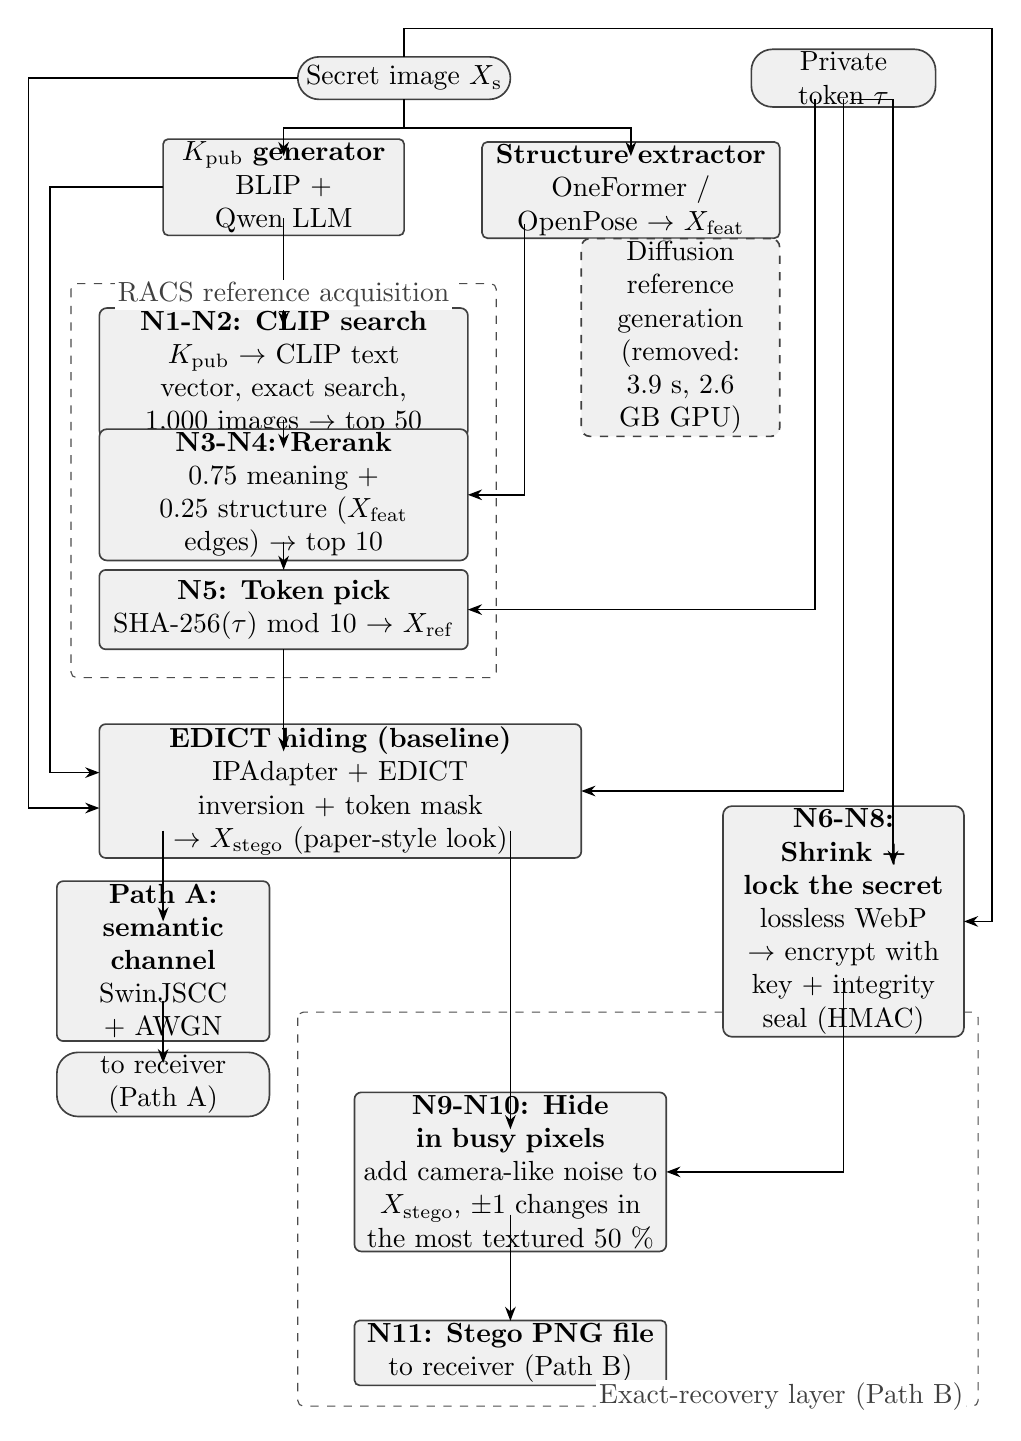
\begin{tikzpicture}
	\hyphenpenalty=10000\exhyphenpenalty=10000
	\draw[dashed, draw=black!70, rounded corners=2pt] (0.720,-3.420) rectangle (6.120,-8.424);
	\draw[dashed, draw=black!70, rounded corners=2pt] (3.600,-12.672) rectangle (12.240,-17.676);
	\node[draw=black!75, fill=black!6, line width=0.6pt, rounded corners=0.095cm, minimum width=4.680cm, minimum height=1.188cm, text width=4.572cm, align=center, inner sep=1pt, font=\diagfont] (3) at (3.420,-4.554) {\textbf{N1-N2: CLIP search} \\ $K_{\mathrm{pub}}$ $\rightarrow$ CLIP text vector, exact search, 1,000 images $\rightarrow$ top 50};
	\node[draw=black!75, fill=black!6, line width=0.6pt, rounded corners=0.095cm, minimum width=4.680cm, minimum height=1.188cm, text width=4.572cm, align=center, inner sep=1pt, font=\diagfont] (4) at (3.420,-6.102) {\textbf{N3-N4: Rerank} \\ 0.75 meaning + 0.25 structure ($X_{\mathrm{feat}}$ edges) $\rightarrow$ top 10};
	\node[draw=black!75, fill=black!6, line width=0.6pt, rounded corners=0.081cm, minimum width=4.680cm, minimum height=1.008cm, text width=4.572cm, align=center, inner sep=1pt, font=\diagfont] (5) at (3.420,-7.560) {\textbf{N5: Token pick} \\ SHA-256($\tau$) mod 10 $\rightarrow$ $X_{\mathrm{ref}}$};
	\node[draw=black!75, fill=black!6, line width=0.6pt, rounded corners=0.087cm, minimum width=3.960cm, minimum height=1.082cm, text width=3.852cm, align=center, inner sep=1pt, font=\diagfont] (8) at (6.300,-14.701) {\textbf{N9-N10: Hide in busy pixels} \\ add camera-like noise to $X_{\mathrm{stego}}$, $\pm$1 changes in the most textured 50 \%};
	\node[draw=black!75, fill=black!6, line width=0.6pt, rounded corners=0.065cm, minimum width=3.960cm, minimum height=0.811cm, text width=3.852cm, align=center, inner sep=1pt, font=\diagfont] (9) at (6.300,-17.000) {\textbf{N11: Stego PNG file} \\ to receiver (Path B)};
	\node[draw=black!75, fill=black!6, line width=0.6pt, rounded corners=0.270cm, minimum width=2.700cm, minimum height=0.540cm, text width=2.592cm, align=center, inner sep=1pt, font=\diagfont] (10) at (4.950,-0.810) {Secret image $X_{\mathrm{s}}$};
	\node[draw=black!75, fill=black!6, line width=0.6pt, rounded corners=0.270cm, minimum width=2.340cm, minimum height=0.540cm, text width=2.232cm, align=center, inner sep=1pt, font=\diagfont] (11) at (10.530,-0.810) {Private token $\tau$};
	\node[draw=black!75, fill=black!6, line width=0.6pt, rounded corners=0.063cm, minimum width=3.060cm, minimum height=0.792cm, text width=2.952cm, align=center, inner sep=1pt, font=\diagfont] (12) at (3.420,-2.196) {\textbf{$K_{\mathrm{pub}}$ generator} \\ BLIP + Qwen LLM};
	\node[draw=black!75, fill=black!6, line width=0.6pt, rounded corners=0.069cm, minimum width=3.780cm, minimum height=0.864cm, text width=3.672cm, align=center, inner sep=1pt, font=\diagfont] (13) at (7.830,-2.232) {\textbf{Structure extractor} \\ OneFormer / OpenPose $\rightarrow$ $X_{\mathrm{feat}}$};
	\node[draw=black!75, fill=black!6, line width=0.6pt, rounded corners=0.109cm, dashed, minimum width=2.520cm, minimum height=1.368cm, text width=2.412cm, align=center, inner sep=1pt, font=\diagfont] (14) at (8.460,-4.104) {Diffusion reference generation (removed: 3.9 s, 2.6 GB GPU)};
	\node[draw=black!75, fill=black!6, line width=0.6pt, rounded corners=0.081cm, minimum width=6.120cm, minimum height=1.008cm, text width=6.012cm, align=center, inner sep=1pt, font=\diagfont] (15) at (4.140,-9.864) {\textbf{EDICT hiding (baseline)} \\ IPAdapter + EDICT inversion + token mask \\ $\rightarrow$ $X_{\mathrm{stego}}$ (paper-style look)};
	\node[draw=black!75, fill=black!6, line width=0.6pt, rounded corners=0.081cm, minimum width=2.700cm, minimum height=1.008cm, text width=2.592cm, align=center, inner sep=1pt, font=\diagfont] (16) at (1.890,-12.024) {\textbf{Path A: semantic channel} \\ SwinJSCC + AWGN};
	\node[draw=black!75, fill=black!6, line width=0.6pt, rounded corners=0.270cm, minimum width=2.700cm, minimum height=0.540cm, text width=2.592cm, align=center, inner sep=1pt, font=\diagfont] (17) at (1.890,-13.590) {to receiver (Path A)};
	\node[draw=black!75, fill=black!6, line width=0.6pt, rounded corners=0.115cm, minimum width=3.060cm, minimum height=1.440cm, text width=2.952cm, align=center, inner sep=1pt, font=\diagfont] (7) at (10.530,-11.520) {\textbf{N6-N8: Shrink + lock the secret} \\ lossless WebP $\rightarrow$ encrypt with key + integrity seal (HMAC)};
	\draw[-{Stealth[length=1.8mm]}, line width=0.6pt] (4.950,-1.080) -- (4.950,-1.440) -- (3.420,-1.440) -- (3.420,-1.800);
	\draw[-{Stealth[length=1.8mm]}, line width=0.6pt] (4.950,-1.080) -- (4.950,-1.440) -- (7.830,-1.440) -- (7.830,-1.800);
	\draw[-{Stealth[length=1.8mm]}, line width=0.6pt] (3.420,-2.592) -- (3.420,-3.960);
	\draw[-{Stealth[length=1.8mm]}, line width=0.6pt] (6.480,-2.664) -- (6.480,-6.102) -- (5.760,-6.102);
	\draw[-{Stealth[length=1.8mm]}, line width=0.6pt] (3.420,-5.148) -- (3.420,-5.508);
	\draw[-{Stealth[length=1.8mm]}, line width=0.6pt] (3.420,-6.696) -- (3.420,-7.056);
	\draw[-{Stealth[length=1.8mm]}, line width=0.6pt] (3.420,-8.064) -- (3.420,-9.360);
	\draw[-{Stealth[length=1.8mm]}, line width=0.6pt] (1.890,-2.196) -- (0.450,-2.196) -- (0.450,-9.630) -- (1.080,-9.630);
	\draw[-{Stealth[length=1.8mm]}, line width=0.6pt] (3.600,-0.810) -- (0.180,-0.810) -- (0.180,-10.080) -- (1.080,-10.080);
	\draw[-{Stealth[length=1.8mm]}, line width=0.6pt] (10.170,-1.080) -- (10.170,-7.560) -- (5.760,-7.560);
	\draw[-{Stealth[length=1.8mm]}, line width=0.6pt] (10.530,-1.080) -- (10.530,-9.864) -- (7.200,-9.864);
	\draw[-{Stealth[length=1.8mm]}, line width=0.6pt] (10.620,-1.080) -- (11.160,-1.080) -- (11.160,-10.800);
	\draw[-{Stealth[length=1.8mm]}, line width=0.6pt] (4.950,-0.540) -- (4.950,-0.180) -- (12.420,-0.180) -- (12.420,-11.520) -- (12.060,-11.520);
	\draw[-{Stealth[length=1.8mm]}, line width=0.6pt] (10.530,-12.240) -- (10.530,-14.701) -- (8.280,-14.701);
	\draw[-{Stealth[length=1.8mm]}, line width=0.6pt] (6.300,-10.368) -- (6.300,-14.160);
	\draw[-{Stealth[length=1.8mm]}, line width=0.6pt] (6.300,-15.242) -- (6.300,-16.594);
	\draw[-{Stealth[length=1.8mm]}, line width=0.6pt] (1.890,-10.368) -- (1.890,-11.520);
	\draw[-{Stealth[length=1.8mm]}, line width=0.6pt] (1.890,-12.528) -- (1.890,-13.320);
	\node[fill=white, inner sep=1pt, font=\diaglabel, text=black!75] at (3.420,-3.564) {RACS reference acquisition};
	\node[anchor=east, fill=white, inner sep=1pt, font=\diaglabel, text=black!75] at (12.096,-17.550) {Exact-recovery layer (Path B)};
\end{tikzpicture}

	\caption{RACS sender (hiding).}
	\label{fig:racs-tx}
\end{figure}

\begin{figure}[H]
	\centering
	% Generated from racs_receiver.drawio by drawio2tikz.py; edit the .drawio file and rerun.
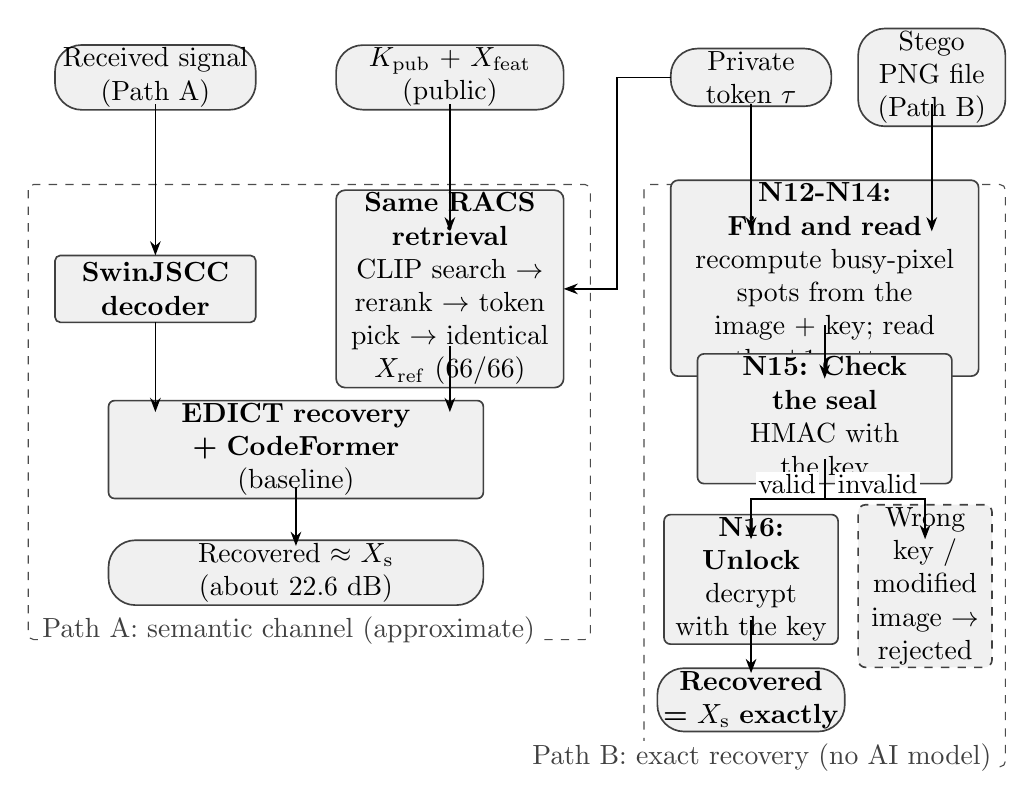
\begin{tikzpicture}
	\hyphenpenalty=10000\exhyphenpenalty=10000
	\draw[dashed, draw=black!70, rounded corners=2pt] (0.340,-2.210) rectangle (7.480,-7.990);
	\draw[dashed, draw=black!70, rounded corners=2pt] (8.160,-2.210) rectangle (12.750,-9.605);
	\node[draw=black!75, fill=black!6, line width=0.6pt, rounded corners=0.068cm, minimum width=2.550cm, minimum height=0.850cm, text width=2.448cm, align=center, inner sep=1pt, font=\diagfont] (dec) at (1.955,-3.536) {\textbf{SwinJSCC decoder}};
	\node[draw=black!75, fill=black!6, line width=0.6pt, rounded corners=0.117cm, minimum width=2.890cm, minimum height=1.462cm, text width=2.788cm, align=center, inner sep=1pt, font=\diagfont] (ret) at (5.695,-3.536) {\textbf{Same RACS retrieval} \\ CLIP search $\rightarrow$ rerank $\rightarrow$ token pick $\rightarrow$ identical $X_{\mathrm{ref}}$ (66/66)};
	\node[draw=black!75, fill=black!6, line width=0.6pt, rounded corners=0.076cm, minimum width=4.760cm, minimum height=0.952cm, text width=4.658cm, align=center, inner sep=1pt, font=\diagfont] (rec) at (3.740,-5.576) {\textbf{EDICT recovery + CodeFormer} \\ (baseline)};
	\node[draw=black!75, fill=black!6, line width=0.6pt, rounded corners=0.340cm, minimum width=4.760cm, minimum height=0.680cm, text width=4.658cm, align=center, inner sep=1pt, font=\diagfont] (oa) at (3.740,-7.140) {Recovered $\approx$ $X_{\mathrm{s}}$ (about 22.6 dB)};
	\node[draw=black!75, fill=black!6, line width=0.6pt, rounded corners=0.095cm, minimum width=3.910cm, minimum height=1.190cm, text width=3.808cm, align=center, inner sep=1pt, font=\diagfont] (find) at (10.455,-3.400) {\textbf{N12-N14: Find and read} \\ recompute busy-pixel spots from the image + key; read the $\pm$1 pattern};
	\node[draw=black!75, fill=black!6, line width=0.6pt, rounded corners=0.082cm, minimum width=3.230cm, minimum height=1.020cm, text width=3.128cm, align=center, inner sep=1pt, font=\diagfont] (seal) at (10.455,-5.185) {\textbf{N15: Check the seal} \\ HMAC with the key};
	\node[draw=black!75, fill=black!6, line width=0.6pt, rounded corners=0.082cm, minimum width=2.210cm, minimum height=1.020cm, text width=2.108cm, align=center, inner sep=1pt, font=\diagfont] (unl) at (9.520,-7.225) {\textbf{N16: Unlock} \\ decrypt with the key};
	\node[draw=black!75, fill=black!6, line width=0.6pt, rounded corners=0.095cm, dashed, minimum width=1.700cm, minimum height=1.190cm, text width=1.598cm, align=center, inner sep=1pt, font=\diagfont] (rej) at (11.730,-7.310) {Wrong key / modified image $\rightarrow$ rejected};
	\node[draw=black!75, fill=black!6, line width=0.6pt, rounded corners=0.340cm, minimum width=2.380cm, minimum height=0.680cm, text width=2.278cm, align=center, inner sep=1pt, font=\diagfont] (ob) at (9.520,-8.755) {\textbf{Recovered = $X_{\mathrm{s}}$ exactly}};
	\node[draw=black!75, fill=black!6, line width=0.6pt, rounded corners=0.340cm, minimum width=2.550cm, minimum height=0.680cm, text width=2.448cm, align=center, inner sep=1pt, font=\diagfont] (recv) at (1.955,-0.850) {Received signal (Path A)};
	\node[draw=black!75, fill=black!6, line width=0.6pt, rounded corners=0.340cm, minimum width=2.890cm, minimum height=0.680cm, text width=2.788cm, align=center, inner sep=1pt, font=\diagfont] (pub) at (5.695,-0.850) {$K_{\mathrm{pub}}$ + $X_{\mathrm{feat}}$ (public)};
	\node[draw=black!75, fill=black!6, line width=0.6pt, rounded corners=0.340cm, minimum width=2.040cm, minimum height=0.680cm, text width=1.938cm, align=center, inner sep=1pt, font=\diagfont] (tau) at (9.520,-0.850) {Private token $\tau$};
	\node[draw=black!75, fill=black!6, line width=0.6pt, rounded corners=0.340cm, minimum width=1.870cm, minimum height=0.680cm, text width=1.768cm, align=center, inner sep=1pt, font=\diagfont] (png) at (11.815,-0.850) {Stego PNG file (Path B)};
	\node[fill=white, inner sep=1pt, font=\diagfont] at (9.979,-6.018) {valid};
	\node[fill=white, inner sep=1pt, font=\diagfont] at (11.127,-6.018) {invalid};
	\draw[-{Stealth[length=1.8mm]}, line width=0.6pt] (1.955,-1.190) -- (1.955,-3.111);
	\draw[-{Stealth[length=1.8mm]}, line width=0.6pt] (5.695,-1.190) -- (5.695,-2.805);
	\draw[-{Stealth[length=1.8mm]}, line width=0.6pt] (8.500,-0.850) -- (7.820,-0.850) -- (7.820,-3.536) -- (7.140,-3.536);
	\draw[-{Stealth[length=1.8mm]}, line width=0.6pt] (1.955,-3.961) -- (1.955,-5.100);
	\draw[-{Stealth[length=1.8mm]}, line width=0.6pt] (5.695,-4.267) -- (5.695,-5.100);
	\draw[-{Stealth[length=1.8mm]}, line width=0.6pt] (3.740,-6.052) -- (3.740,-6.800);
	\draw[-{Stealth[length=1.8mm]}, line width=0.6pt] (9.520,-1.190) -- (9.520,-2.805);
	\draw[-{Stealth[length=1.8mm]}, line width=0.6pt] (11.815,-1.190) -- (11.815,-2.805);
	\draw[-{Stealth[length=1.8mm]}, line width=0.6pt] (10.455,-3.995) -- (10.455,-4.675);
	\draw[-{Stealth[length=1.8mm]}, line width=0.6pt] (10.455,-5.695) -- (10.455,-6.205) -- (9.520,-6.205) -- (9.520,-6.715);
	\draw[-{Stealth[length=1.8mm]}, line width=0.6pt] (10.455,-5.695) -- (10.455,-6.205) -- (11.730,-6.205) -- (11.730,-6.715);
	\draw[-{Stealth[length=1.8mm]}, line width=0.6pt] (9.520,-7.735) -- (9.520,-8.415);
	\node[anchor=west, fill=white, inner sep=1pt, font=\diaglabel, text=black!75] at (0.476,-7.871) {Path A: semantic channel (approximate)};
	\node[anchor=east, fill=white, inner sep=1pt, font=\diaglabel, text=black!75] at (12.614,-9.486) {Path B: exact recovery (no AI model)};
\end{tikzpicture}

	\caption{RACS receiver (recovery).}
	\label{fig:racs-rx}
\end{figure}

\paragraph{The reference is found, not painted.} The public key $K_{\mathrm{pub}}$ is turned into
a CLIP embedding and used to search a fixed collection of 1{,}000 images. The 50 closest images
are re-scored by how well they match in meaning (75\,\%) and in layout (25\,\%, comparing edge
maps with the public structure $X_{\mathrm{feat}}$), and the token picks one of the best 10. The
receiver repeats exactly the same steps from public data and the token and gets exactly the same
image (66 of 66 test images), in 0.05\,s and without a GPU.

\paragraph{The secret arrives exactly.} The stego image still travels through the semantic
channel (Path A), giving an approximate recovery as in the baseline. In addition, the original
secret is compressed losslessly, encrypted and sealed with a key derived from the token, and
hidden with tiny $\pm1$ changes in the most textured pixels of the stego image, which is sent as a
PNG file (Path B). The receiver recomputes the same pixel positions, checks the seal and decrypts.
A wrong key or an altered file is rejected instead of producing a misleading image.

\section{New-Block Reference}
\begin{table}[!htbp]
	\centering
	\caption{New RACS blocks (labels as in Figures~\ref{fig:racs-tx} and~\ref{fig:racs-rx}) and the reason for each design choice.}
	\label{tab:newblocks}
	\begin{tabularx}{\textwidth}{|c|l|X|}
		\hline
		\textbf{Block} & \textbf{What it does} & \textbf{Design choice and reason} \\ \hline
		N1 & CLIP text embedding of $K_{\mathrm{pub}}$ & Query from \emph{public} data only, so the receiver can recompute it without the secret. \\ \hline
		N2 & Exact search, top-50 pool & No approximate index, so sender and receiver get identical rankings. \\ \hline
		N3 & Edge-map structural score & CLIP finds the right content but not the right layout; $X_{\mathrm{feat}}$ is the only public structure both sides hold. \\ \hline
		N4 & 0.75 / 0.25 rerank, top 10 & Weights chosen on calibration images only; reranking a wider pool changes \emph{which} images the token can pick. \\ \hline
		N5 & SHA-256($\tau$) mod $K$ & One implementation at both ends; a 1-in-$K$ guess for an attacker. \\ \hline
		N6 & Lossless WebP compaction & 32\,\% smaller payload, which makes a low embedding rate affordable. \\ \hline
		N7 & PBKDF2 key derivation \cite{rfc8018} & Slows brute force of the short numeric token. \\ \hline
		N8, N16 & Stream encryption \cite{fips202} & Hidden bits look random. \\ \hline
		N8, N15 & HMAC-SHA256 seal \cite{rfc2104} & A wrong key or modified image is \emph{rejected}, never shown as a wrong image. \\ \hline
		N9 & Carrier upscale + dither & An upscaled image has an unnaturally clean LSB plane; camera-like noise makes it realistic. \\ \hline
		N10, N13 & Texture-adaptive $\pm1$ & Changes only busy regions; $\pm1$ instead of overwriting defeats the chi-square attack; the receiver recomputes positions with no side information. \\ \hline
		N11, N12 & PNG file transfer & Lossless; recompression would destroy the payload (and is detected). \\ \hline
	\end{tabularx}
\end{table}

\paragraph{One change at a time.} In the code, RACS is a subclass of the baseline that
overrides a single method: where the reference comes from. Every other stage is imported, not
copied, so any measured difference comes from the reference alone.

\section{Prototype Architecture}
\begin{figure}[H]
	\centering
	\begin{tikzpicture}[scale=0.85, transform shape]
		\node[src, text width=2.4cm] (s) at (0,0) {Sender phone\\(browser)};
		\node[blk, text width=3.0cm] (srv) at (5.2,0) {Laptop web server\\(runs the pipeline)};
		\node[src, text width=2.4cm] (r) at (10.4,0) {Receiver phone\\(browser)};
		\node[newblk, text width=3.4cm] (w) at (5.2,-2.0) {Worker process\\public key + RACS retrieval};
		\draw[arr] (s) -- node[above, font=\scriptsize]{secret photo} (srv);
		\draw[arr] (srv) -- node[above, font=\scriptsize]{stego PNG + key} (r);
		\draw[arr, <->] (srv) -- (w);
	\end{tikzpicture}
	\caption{Phone prototype: phones connect over Wi-Fi and the laptop does all the work.}
	\label{fig:app}
\end{figure}

The prototype offers three modes: \emph{hybrid} (default: diffusion stego look plus the exact
layer), \emph{lossless} (exact layer on a retrieved cover, no diffusion) and \emph{diffusion}
(the paper's approximate pipeline). The stego must be sent as a file, because messaging apps
recompress photos; the receiver detects this through the seal.

\section{Code Organisation}
\begin{table}[H]
	\centering
	\caption{Modules of the implementation.}
	\label{tab:modules}
	\begin{tabularx}{\textwidth}{|l|X|}
		\hline
		\textbf{Package} & \textbf{Responsibility} \\ \hline
		\texttt{common} & Paths, seeding, device selection, low-memory model loading \\ \hline
		\texttt{configs} & One configuration file read by both ends \\ \hline
		\texttt{semantic} & Public key and structure extraction \\ \hline
		\texttt{reference} & Baseline reference generation and ControlNet fine-tuning \\ \hline
		\texttt{retrieval} & RACS: corpus, search, structure cache, rerank, token pick \\ \hline
		\texttt{steganography} & EDICT, hiding, recovery, token mask, IPAdapter \\ \hline
		\texttt{communication} & AWGN channel and SwinJSCC codec \\ \hline
		\texttt{enhancement} & CodeFormer face restoration \\ \hline
		\texttt{pipelines} & The assembled baseline and RACS systems \\ \hline
		\texttt{evaluation} & Metrics, frozen test splits, reports \\ \hline
		\texttt{security} & Token tests, XuNet, chi-square and SPA detectors \\ \hline
		\texttt{app} & Phone web server and the exact-recovery layer \\ \hline
		\texttt{scripts} & Build and verification script for every phase \\ \hline
	\end{tabularx}
\end{table}

        \chapter{Implementation}
        The system was built incrementally in phases. Each phase had a stated goal, a small
experiment, an artifact saved to disk and a verification gate (Section~\ref{sec:gates}). This
chapter describes the phases in order, then the engineering problems that shaped the
implementation.

\section{Methodology}
The working rule was \emph{baseline first}: no RACS component was wired into the pipeline until
the reproduced baseline passed its gate, so the comparison in Chapter~6 is against a measured
baseline rather than against numbers copied from the paper. Every phase followed the same loop:
state what is built and why; build the smallest experiment; test it; explain the output;
integrate; save the artifact with its configuration hash; move on.

\begin{figure}[H]
	\centering
	\begin{tikzpicture}[scale=0.85, transform shape]
		\hyphenpenalty=10000\exhyphenpenalty=10000
		% baseline milestones, left to right
		\node[blk, text width=2.3cm] (m1) at (0,0) {\textbf{Phases 1--3}\\environment, VAE, diffusion cost};
		\node[blk, text width=2.3cm] (m2) at (3.0,0) {\textbf{Phases 4--6}\\corpus, CLIP, frozen splits};
		\node[blk, text width=2.3cm] (m3) at (6.0,0) {\textbf{Phases 7--9}\\$K_{\mathrm{pub}}$, $X_{\mathrm{feat}}$, references};
		\node[blk, text width=2.3cm] (m4) at (9.0,0) {\textbf{Phases 10--14}\\EDICT, hiding, channel, CodeFormer};
		\node[blk, text width=2.3cm] (m5) at (12.0,0) {\textbf{Phases 15--16}\\baseline frozen: quality, security};
		% RACS milestones, right to left underneath
		\node[newblk, text width=2.3cm] (m6) at (12.0,-3.0) {\textbf{Phases 17--20}\\retrieval, token pick, rerank};
		\node[newblk, text width=2.3cm] (m7) at (9.0,-3.0) {\textbf{Phases 21--22}\\RACS end to end, comparison};
		\node[newblk, text width=2.3cm] (m8) at (6.0,-3.0) {\textbf{Exact layer}\\lossless, sealed, adaptive embedding};
		\node[src, text width=2.3cm] (m9) at (3.0,-3.0) {Phone prototype};
		\draw[arr] (m1) -- (m2);
		\draw[arr] (m2) -- (m3);
		\draw[arr] (m3) -- (m4);
		\draw[arr] (m4) -- (m5);
		\draw[arr] (m5) -- node[left, font=\scriptsize, align=right]{baseline gate\\passed} (m6);
		\draw[arr] (m6) -- (m7);
		\draw[arr] (m7) -- (m8);
		\draw[arr] (m8) -- (m9);
		\node[font=\footnotesize\bfseries, text=gray!50!black, anchor=south west] at ([yshift=0.15cm]m1.north west) {Baseline reproduction (AgentSemSteCom)};
		\node[font=\footnotesize\bfseries, text=green!35!black, anchor=north west] at ([yshift=-0.15cm]m9.south west) {RACS};
	\end{tikzpicture}
	\caption{Order of work. Every phase ends with an artifact and an automatic verification gate; nothing RACS-specific was wired in before the baseline gate passed.}
	\label{fig:phases}
\end{figure}

\section{Foundation (Phases 1--3)}
\subsection{Phase 1: environment and tensor contract}
A virtual environment with PyTorch~2.6 and CUDA~12.4 was created, and all model caches were
redirected to the data drive. A seeding utility fixes Python, NumPy and PyTorch (CPU and CUDA)
random states. The tensor contract was fixed: images are RGB, \texttt{float32}, shape
$(1,3,H,W)$, values in $[0,1]$ for metrics and $[-1,1]$ for the VAE. The gate checks CUDA
availability, configuration loading, tensor shapes and that two seeded runs produce identical
tensors.

\subsection{Phase 2: VAE and latent space}
The Stable Diffusion VAE compresses a $512\times512\times3$ image to a $64\times64\times4$ latent
(an $8\times$ spatial reduction). A round trip over five test images gave a mean PSNR of
32.81\,dB (range 31.78--34.15) and SSIM 0.935. This sets a ceiling: any pipeline that passes
through the VAE cannot recover a secret better than about 33\,dB.


\subsection{Phase 3: diffusion generation cost}
Stable Diffusion v1.5 was loaded in half precision with attention slicing and a DDIM scheduler.
A sweep over steps and seeds measured cost: at 20 steps one $512$\,px image took 5.56\,s
(0.278\,s per step) with 2.60\,GB peak GPU memory, so the paper's 50 steps cost 13.5\,s per
image. Disabling classifier-free guidance reduced cost by a factor of 1.73, confirming that the
UNet forward pass dominates. Cost grows linearly with the number of denoising steps (5.56,
8.18 and 13.47\,s at 20, 30 and 50 steps), which is exactly the per-message cost that RACS removes.

\section{Retrieval Inputs and Test Harness (Phases 4--6)}
\subsection{Phase 4: retrieval corpus}
A builder deterministically sampled 1{,}000 images from COCO val2017 with a fixed seed,
centre-cropped and resized them to $512\times512$ RGB, and wrote a versioned index file listing
each image identifier, path and SHA-256 hash. The row order of this file is part of the protocol,
because the index returns row numbers. The verification gate checks every hash, the row count
and that a rebuild is identical.


\subsection{Phase 5: CLIP embeddings}
CLIP ViT-B/32 embeds each corpus image to a 512-dimensional, L2-normalised \texttt{float32}
vector. Embeddings are kept in single precision because half precision changed nearest-neighbour
orderings in borderline cases. Re-encoding the corpus gave a maximum absolute difference of
$2.5\times10^{-7}$. Using COCO captions as queries, the correct image was the top-1 result 47.6\,\%
of the time out of 1{,}000; mean similarity was 0.779 within a topic and 0.542 across topics.


An important observation was that CLIP similarity and structural similarity disagree: two
images can be semantically close but laid out completely differently (in one case, CLIP
similarity 0.643 but edge overlap only 0.199). This motivated the structural reranking of Phase 20.


\subsection{Phase 6: evaluation harness and frozen splits}
Two frozen, role-tagged splits were built (Section~3.7). The calibration split (UniStega, 22 per
class) may only be used to check the paper's regime and to tune parameters; the evaluation split
(COCO, Commons portraits, Commons cats, 22 per class, disjoint from the corpus) is the only
source of claims. The split module refuses to return evaluation data to a tuning routine.
Each image is assigned a fixed token stored in a versioned token file. The facial evaluation
images were filtered by title and by CLIP to keep only real single-face photographs. Metrics
(MSE, PSNR, SSIM, LPIPS with an AlexNet backbone) and a frozen report schema were implemented, and
a self-test with 83 checks verifies them.

\section{Baseline Reproduction (Phases 7--16)}
\subsection{Phase 7: public conditions}
For each of the 132 split images, BLIP produces a perception caption with greedy decoding, and
Qwen2.5-0.5B-Instruct rewrites it into a concise generation prompt using a fixed one-shot chat
template. The reply is sanitised (instruction echoes, markdown and URLs removed); a degenerate
reply falls back deterministically to the perception caption, and the number of fallbacks is
recorded (zero occurred). OneFormer produces 150-class ADE20K segmentation for common images.
OpenPose produces body and face keypoints for portraits; on 3 of the 22 tightly cropped
evaluation portraits OpenPose detects no body, and a MediaPipe face mesh is used instead, with
the method recorded per image. To fit in memory, the build runs in two passes (all prompts, then
all features) with one model resident at a time.

\subsection{Phase 8: reference generation}
PicX-Real with the Stable Diffusion v1.5 segmentation and OpenPose ControlNets generates one
reference per image at $256$\,px with 20 DDIM steps and guidance 7.5, from a token-derived seed.
Two independent runs produced byte-identical images for all 132 references (peak GPU memory
2.84\,GB). The IPAdapter-plus image embedding of each reference is precomputed on the CPU and
cached on disk keyed by the reference's SHA-256, so both ends read an identical tensor and the
2.5\,GB image encoder never has to share the GPU with Stable Diffusion.


\subsection{Phase 9: ControlNet zero-convolution fine-tuning}
Algorithm~2 of the paper fine-tunes only the zero-convolution layers of ControlNet. A short run
(50 steps, batch 1, \texttt{bfloat16}, calibration data only) was performed to validate the code
path; half precision produced NaN gradients within five steps, while \texttt{bfloat16} was stable.
A held-out probe loss improved from 0.1488 to 0.1296.

\subsection{Phase 10: EDICT}
EDICT was implemented from the coupled-transformation equations as its own module and tested in
isolation by inverting and regenerating random and image latents across a sweep of step counts
and mixing coefficients. At the operating point (20 steps, $p=0.93$,
half-precision UNet with single-precision latents) the maximum relative latent error was
$3.6\times10^{-3}$: a numerical floor from half precision, not an algorithmic failure. The sweep
also exposed a latent bug: the configuration included $p=0.5$, at which the coupling is
singular, so a full rebuild could never finish. The sweep now starts at 0.55.

\subsection{Phase 11: local hiding and recovery}
A full inversion treats the clean secret latent as pure noise and decodes to a reference-like
image (11.3\,dB against the secret), which is not imperceptible. Hiding therefore uses a
bounded-strength EDICT chain (strength 0.2, 20 steps, guidance 3.0) that is still an exact
paired inverse. Token noise and the sparse token mask are applied in the latent. IPAdapter
injects the reference embedding at both ends, making the stego depend on the reference pixels.

\subsection{Phase 12: AWGN channel}
The channel adds Gaussian noise whose strength is set from the signal power and the target
SNR, split equally across the in-phase and quadrature parts of complex symbols. A seeded generator
provides the noise realisation so that experiments are repeatable. The measured noise variance
matched the analytic value within 0.46\,\%.

\subsection{Phase 13: semantic codec}
The official SwinJSCC release with bandwidth $C=64$ trained at 10\,dB (the nearest public
checkpoint to the paper's $C=48$) was integrated in single precision, with only its noise
generator replaced by a seeded one. In isolation it reconstructs images at 32.54\,dB at 10\,dB
SNR, compared with 22.88\,dB for the VAE-based substitute used before the official weights were
obtained.

\subsection{Phase 14: CodeFormer enhancement}
The official CodeFormer architecture and checkpoint run at $512$\,px with fidelity 0.5 on the
facial class only, on the CPU because of GPU memory. The gate requires measured deltas rather
than assuming improvement; CodeFormer may lower PSNR slightly while improving LPIPS.

\subsection{Phase 15: assembled baseline}
The stages were assembled into one baseline object. A calibration run (15A) checks the regime
against the paper's Table~II with tolerances (Gate~A), and an evaluation run (15B) produces the
frozen table (Gate~B). The manifest records the configuration hash, split and token versions,
and the hash of every model. Results are in Chapter~6.

\subsection{Phase 16: security and steganalysis}
Recovery is measured under three receiver conditions: the \emph{correct} token, a valid
\emph{wrong} token, and \emph{no token} (a fixed public fallback token with an all-zero mask).
A XuNet steganalyser with a fixed SRM high-pass first layer is trained to separate clean images
from stego images, with the train, validation and test splits grouped by image so that patches of
one image never cross splits.

\section{RACS Reference Retrieval (Phases 17--22)}
All retrieval logic lives in one module shared by transmitter and receiver.

\subsection{Phase 17: exact retrieval}
The corpus embeddings are indexed with an exact inner-product index. A FAISS
\texttt{IndexFlatIP} is built and saved in its own process; within the pipeline, the same exact
inner product is computed with NumPy, because FAISS and PyTorch load conflicting OpenMP runtimes
in one process on Windows. The gate verifies that FAISS and the in-process search return identical
top-50 rows and scores, that each corpus image retrieves itself first with score 1.0, and that the
row order matches the index file.

\subsection{Phase 18: token selection}
The token is hashed with SHA-256 together with a fixed label, and the result modulo $K$
gives the position of the chosen image in the top-$K$ list. The gate verifies identical output in separate processes, that $K=1$ always selects index 0, that
over the evaluation tokens all ten buckets are used and the distribution is near uniform, and
that the language's built-in hash is never called.

\subsection{Phase 19: structural representation}
Each corpus image is converted to a dilated binary edge map at $128$\,px and cached. Query
structure is derived from the public $X_{\mathrm{feat}}$ (segment boundaries or keypoint
coverage). The cache is deterministic, and the gate requires at least three cases in which the
CLIP ranking and the structural ranking disagree; five were found.

\subsection{Phase 20: reranking}
Each candidate gets a combined score: a weight $\alpha$ times its CLIP similarity plus a weight
$\beta$ times its edge-map overlap with the public structure. A sweep on
calibration data only measured, for the selected top-10 pool, the mean semantic similarity to the
secret, the mean edge IoU, and the fraction of images whose pool changed relative to CLIP alone
(Figure~\ref{fig:sweep}). The objective weights semantic similarity and edge IoU equally.

\begin{figure}[H]
	\centering
	\begin{tikzpicture}
		\begin{axis}[viz, width=0.75\textwidth, height=5.4cm,
			xlabel={Semantic weight $\alpha$ \ (structural weight $\beta = 1-\alpha$)},
			ylabel={Calibration objective},
			xtick={0,0.25,0.5,0.75,1}, xmin=-0.08, xmax=1.08,
			ymin=0.762, ymax=0.7745,
			yticklabel style={/pgf/number format/fixed, /pgf/number format/precision=3}]
			\addplot[vizA, mark=*, mark size=2pt] coordinates {(0,0.7648) (0.25,0.7690) (0.5,0.7717) (0.75,0.7723) (1,0.7640)};
			\addplot[only marks, mark=*, mark size=3.6pt, vizB, forget plot] coordinates {(0.75,0.7723)};
			\node[font=\scriptsize, anchor=south, text=black] at (axis cs:0.75,0.7726) {chosen: $\alpha=0.75$};
		\end{axis}
	\end{tikzpicture}
	\caption{Rerank weight sweep on calibration data only. Mixing in some structure beats pure CLIP ranking; $\alpha=0.75$ scores best and changes the top-10 pool for two thirds of the images.}
	\label{fig:sweep}
\end{figure}

$\alpha = 0.75$, $\beta = 0.25$ maximises the objective; it keeps most of the semantic quality of
CLIP alone while raising structural agreement, and it changes the candidate pool for two thirds
of the images. These weights were frozen before any evaluation run.

\subsection{Phase 21: RACS end to end}
RACS-Base subclasses the baseline and overrides only reference acquisition. Retrieval for the
transmitter and for the receiver run in two separate processes before the diffusion stack loads
(CLIP text encoding crashed when loaded beside it). The gate requires
$X_{\mathrm{ref}}^{\mathrm{tx}} = X_{\mathrm{ref}}^{\mathrm{rx}}$ for every evaluation image, compared
by identifier and file hash. Both systems are then measured through the same object and the same
evaluation function, differing only in where the reference comes from.

\subsection{Phase 22: controlled comparison}
A comparison script reads both systems' measurements on the same cases and tokens, refuses
calibration data, and reports quality, security, latency and memory side by side (Chapter~6).

\section{RACS Exact-Recovery Layer}
The layer is a self-contained module with four functions: compaction,
carrier preparation, embedding and extraction. A container
format stores a magic value, the length and the format of the payload, and the HMAC tag.
Evaluation generates 66 paper-style carriers (EDICT at strength 0.5 with a RACS-retrieved
reference), embeds every evaluation secret with four progressively stronger variants, writes each
stego to a real PNG file and reads it back before extraction. Two classical detectors were
implemented: Westfeld's chi-square test and Sample Pair Analysis. For each detector the AUC is
computed between each stego and the same carrier without payload, so 0.5 means the detector cannot
tell them apart.

Figure~\ref{fig:payload} shows how one secret becomes the hidden bit stream. The token is
stretched once by PBKDF2 into three independent values: an encryption key, a MAC key and the seed
that orders the embedding positions. Because the positions are chosen from texture computed on the
top five bits of each value, and a $\pm1$ change never alters those bits, the receiver recomputes
exactly the same positions from the stego image alone.

\begin{figure}[H]
	\centering
	\begin{tikzpicture}[scale=0.8, transform shape]
		\hyphenpenalty=10000\exhyphenpenalty=10000
		% key schedule (row 1)
		\node[src, text width=2.0cm] (tok) at (0,0) {Token $\tau$};
		\node[newblk, text width=2.4cm] (kdf) at (3.0,0) {\textbf{PBKDF2}\\200{,}000 rounds};
		\node[draw, thick, minimum height=0.8cm, minimum width=2.3cm, fill=gray!8, font=\footnotesize, anchor=west] (ek) at (5.4,0) {encryption key};
		\node[draw, thick, minimum height=0.8cm, minimum width=1.6cm, fill=gray!8, font=\footnotesize, right=0pt of ek] (mk) {MAC key};
		\node[draw, thick, minimum height=0.8cm, minimum width=2.1cm, fill=gray!8, font=\footnotesize, right=0pt of mk] (ps) {position seed};
		% payload container (row 2)
		\node[src, text width=2.0cm] (sec) at (0,-2.0) {Secret file};
		\node[newblk, text width=2.4cm] (cmp) at (3.0,-2.0) {\textbf{Compact}\\lossless WebP if smaller};
		\node[draw, thick, minimum height=0.8cm, minimum width=1.0cm, fill=gray!8, font=\footnotesize, anchor=west] (hdr) at (5.4,-2.0) {RACS};
		\node[draw, thick, minimum height=0.8cm, minimum width=1.1cm, fill=gray!8, font=\footnotesize, right=0pt of hdr] (len) {length};
		\node[draw, thick, minimum height=0.8cm, minimum width=1.8cm, fill=green!12, font=\footnotesize, right=0pt of len] (body) {file bytes};
		\node[src, text width=2.0cm] (png) at (13.0,-2.0) {Stego PNG};
		% processing (row 3)
		\node[newblk, text width=2.4cm] (enc) at (6.6,-4.1) {\textbf{Encrypt}\\SHAKE-256 stream (encryption key)};
		\node[newblk, text width=2.4cm] (mac) at (9.8,-4.1) {\textbf{Seal}\\32-byte HMAC tag (MAC key)};
		\node[newblk, text width=2.6cm] (emb) at (13.0,-4.1) {\textbf{Embed}\\$\pm1$ in most textured 50\,\% (position seed)};
		\draw[arr] (tok) -- (kdf);
		\draw[arr] (kdf) -- (ek);
		\draw[arr] (sec) -- (cmp);
		\draw[arr] (cmp) -- (hdr);
		\draw[arr] (len.south) -- (len.south |- enc.north);
		\draw[arr] (enc) -- (mac);
		\draw[arr] (mac) -- (emb);
		\draw[arr] (emb) -- (png);
	\end{tikzpicture}
	\caption{How the exact-recovery layer packs a secret. The token is stretched into three independent values, each used by one step; a wrong token produces a different MAC key, so the seal check fails and the file is rejected.}
	\label{fig:payload}
\end{figure}

\section{Prototype}
A web server on the laptop serves a mobile page. The sender uploads a photograph and receives a
stego PNG and an 8-digit key; the receiver uploads the PNG and the key and receives the secret.
Photographs keep their aspect ratio by edge-padding to a square at $512$\,px and cropping back on
receipt. The public-key generation and retrieval run in a separate worker process for the reasons
given above. A self-test mode runs a round trip from the command line. Figure~\ref{fig:sequence}
shows one complete exchange.

\begin{figure}[H]
	\centering
	\begin{tikzpicture}[scale=0.85, transform shape]
		\hyphenpenalty=10000\exhyphenpenalty=10000
		% participants
		\node[src, text width=2.4cm] (s) at (0,0) {\textbf{Sender phone}};
		\node[blk, text width=2.6cm] (l) at (5.5,0) {\textbf{Laptop server}};
		\node[src, text width=2.4cm] (r) at (11,0) {\textbf{Receiver phone}};
		\foreach \n in {s,l,r} \draw[dashed, gray!70] (\n.south) -- ++(0,-9.2);
		% send
		\draw[arr] (0,-1.1) -- node[above, font=\footnotesize]{upload secret photo} (5.5,-1.1);
		\node[newblk, text width=3.6cm, font=\footnotesize] at (5.5,-2.1) {$K_{\mathrm{pub}}$, RACS retrieval, EDICT stego look, encrypt + embed};
		\draw[arr] (5.5,-3.5) -- node[above, font=\footnotesize]{stego PNG + 8-digit key} (0,-3.5);
		% hand-over between people
		\draw[arr] (0,-4.4) -- node[above, font=\footnotesize]{PNG sent as a file (any messenger)} (11,-4.4);
		\draw[arr, dashed] (0,-5.1) -- node[above, font=\footnotesize]{key shared separately} (11,-5.1);
		% receive
		\draw[arr] (11,-6.0) -- node[above, font=\footnotesize]{upload PNG + key} (5.5,-6.0);
		\node[newblk, text width=3.6cm, font=\footnotesize] at (5.5,-7.0) {read $\pm1$ bits, check seal, decrypt (no AI model)};
		\draw[arr] (5.5,-8.2) -- node[above, font=\footnotesize]{exact secret, or ``rejected''} (11,-8.2);
	\end{tikzpicture}
	\caption{One exchange in the phone prototype. The laptop does all computation; a recompressed photo or a wrong key is detected by the seal and rejected.}
	\label{fig:sequence}
\end{figure}

\section{Verification Results}
Every phase writes its gate result to a JSON record of named checks, so the state of the whole
build can be audited at any time. Figure~\ref{fig:gates} summarises the stored records: 119 checks
across twelve phases, 113 of which pass. All six failures sit in Phases 15 and 16 and have a
single cause: those phases were run on the 2-image-per-class subset, while their gates expect the
full 22 images per class (sample counts, record counts, and the hash of the full frozen table).
Every determinism, provenance and component check passes, including all RACS phases.

\begin{figure}[H]
	\centering
	\begin{tikzpicture}
		\begin{axis}[vizbar, ybar stacked, bar width=13pt, width=0.95\textwidth, height=5.6cm,
			symbolic x coords={5,7,8,9,10,15,16,17,18,19,20,21}, xtick=data,
			xlabel={Phase}, ylabel={Verification checks}, ymin=0, ymax=22,
			enlarge x limits=0.05,
			legend style={at={(0.98,0.97)}, anchor=north east}]
			\addplot[fill=green!55!black, draw=none] coordinates {(5,20) (7,13) (8,12) (9,10) (10,14) (15,11) (16,12) (17,6) (18,5) (19,3) (20,3) (21,4)};
			\addplot[fill=red!70!black, draw=none] coordinates {(5,0) (7,0) (8,0) (9,0) (10,0) (15,1) (16,5) (17,0) (18,0) (19,0) (20,0) (21,0)};
			\legend{Passed, Failed (subset size only)}
		\end{axis}
	\end{tikzpicture}
	\caption{Automatic verification checks per phase, from the stored gate records. Phases 17--21 are the RACS phases.}
	\label{fig:gates}
\end{figure}

\section{Engineering Challenges}
\begin{itemize}
	\item \textbf{Windows commit charge.} Memory-mapped checkpoint loading reserved more virtual
	memory than the paging file allowed, causing access violations. A small shim loads
	\texttt{safetensors} files read-only before any model library is imported.
	\item \textbf{6\,GB GPU.} Half precision, attention slicing, $256$\,px operation, one model
	resident at a time, CPU placement of the IPAdapter encoder and CodeFormer, and on-disk caches
	of derived tensors kept every phase within budget.
	\item \textbf{Cross-process determinism.} Process-randomised hashing, half-precision encoders
	and implicit device nondeterminism were removed from every path that affects the reference.
	\item \textbf{Float-to-integer truncation.} A conversion on the transmitter side truncated
	instead of rounding before the IPAdapter embedding, which could have desynchronised the two
	ends; caching by reference hash removed the risk.
	\item \textbf{Mixed-state detection.} Upgrading components invalidated earlier frozen
	artifacts. Configuration and model hashes in every manifest made the verification gates fail
	loudly until the affected phases were rebuilt, instead of silently mixing results.
\end{itemize}

        \chapter{Results}
        This chapter reports measured results. All numbers come from the evaluation split unless
labelled \emph{calibration}; paper values are shown only as anchors and are never mixed into
measured rows.

\section{Experimental Setup}
\begin{itemize}
	\item \textbf{Classes.} Common (COCO scenes), facial (portraits), style (cat photographs).
	\item \textbf{Channel.} SwinJSCC ($C=64$) over AWGN at 5, 10, 15 and 20\,dB SNR.
	\item \textbf{Hiding.} EDICT, 20 steps, strength 0.2, mixing 0.93, $\eta = 0.05$, IPAdapter-plus
	weight 1, $256$\,px.
	\item \textbf{Sample sizes.} The baseline and the RACS comparison were measured on 2 images per
	class at all four SNRs (24 cases per system); the transmitter--receiver invariant and the
	exact-recovery layer were measured on all 66 evaluation images.
\end{itemize}

\section{Baseline Recovery Quality}
\begin{table}[H]
	\centering
	\caption{Baseline recovery PSNR (dB) by class and SNR.}
	\label{tab:basepsnr}
	\begin{tabular}{|l|c|c|c|c|}
		\hline
		\textbf{Class} & \textbf{5 dB} & \textbf{10 dB} & \textbf{15 dB} & \textbf{20 dB} \\ \hline
		Common & 18.30 & 20.72 & 21.53 & 21.45 \\ \hline
		Facial & 22.56 & 24.53 & 24.89 & 25.10 \\ \hline
		Style & 19.93 & 22.68 & 23.28 & 23.43 \\ \hline
	\end{tabular}
\end{table}

Quality rises with SNR and flattens above 15\,dB, where the channel stops being the bottleneck and
the VAE and diffusion round trip limit quality. The perceptual metrics follow the same pattern:
from 5 to 20\,dB, SSIM improves from 0.42--0.60 to 0.58--0.72 and LPIPS falls from 0.23--0.46 to
0.14--0.24 across the three classes. Faces score highest, helped by CodeFormer.
Against the paper's Table~II anchors, the facial class at 5\,dB reaches 22.56\,dB (paper 22.73)
and at 20\,dB 25.10\,dB with LPIPS 0.140 (paper 26.29\,dB, LPIPS 0.213); the common class at
5\,dB reaches 18.30\,dB (paper 19.71); the style class at 5\,dB has LPIPS 0.345 (paper 0.385).
Absolute PSNR is about 1--3\,dB below the paper, consistent with the reduced resolution, step
count and strength forced by the hardware (Section~\ref{sec:deviations}).

\section{Baseline Security and Steganalysis}
\begin{table}[H]
	\centering
	\caption{Recovery PSNR under the three receiver conditions (10\,dB).}
	\label{tab:security}
	\begin{tabular}{|l|c|c|}
		\hline
		\textbf{Condition} & \textbf{This work} & \textbf{Paper (approx.)} \\ \hline
		Correct token & 22.37 dB & 25.37 dB \\ \hline
		Wrong token & 13.96 dB & 18.91 dB \\ \hline
		No token & 14.02 dB & -- \\ \hline
		\textbf{Correct $-$ wrong gap} & \textbf{8.41 dB} & 6.46 dB \\ \hline
		XuNet detection accuracy & 0.500 & 0.509 \\ \hline
	\end{tabular}
\end{table}

A wrong or missing token reduces recovery to about 14\,dB, an unrecognisable image. The gap
between correct and wrong token is larger than in the paper, so a wrong key reveals less. XuNet is
at chance, so this detector cannot distinguish stego images from clean ones.

\section{RACS versus the Baseline}
\subsection{Protocol invariant}
In separate transmitter and receiver processes, RACS selected the same reference for
\textbf{66 of 66} evaluation images, with identical file hashes. The FAISS index and the
in-process exact search returned identical top-50 rows and scores.

\subsection{Efficiency}
Obtaining the reference is the stage RACS replaces, and it is where the difference is largest
(Figure~\ref{fig:eff}). Diffusion generation takes 3.92\,s and 2.61\,GB of GPU memory per
reference; retrieval takes 0.048\,s (0.51\,s including loading the image from disk) and needs no
GPU at all, about $82\times$ faster. Because both ends must obtain the reference for every message,
the saving applies twice per message.

\begin{figure}[H]
	\centering
	\begin{subfigure}{0.48\textwidth}
		\centering
		\begin{tikzpicture}
			\begin{axis}[vizbar, xbar, bar width=12pt, width=\textwidth, height=3.8cm,
				symbolic y coords={RACS,Baseline}, ytick=data, enlarge y limits=0.5,
				xmin=0, xmax=5, xlabel={Seconds per reference},
				nodes near coords, nodes near coords style={font=\scriptsize, /pgf/number format/fixed, /pgf/number format/precision=3}]
				\addplot[fill=vizA, draw=none] coordinates {(3.92,Baseline) (0.048,RACS)};
			\end{axis}
		\end{tikzpicture}
		\caption{Reference latency.}
	\end{subfigure}\hfill
	\begin{subfigure}{0.48\textwidth}
		\centering
		\begin{tikzpicture}
			\begin{axis}[vizbar, xbar, bar width=12pt, width=\textwidth, height=3.8cm,
				symbolic y coords={RACS,Baseline}, ytick=data, enlarge y limits=0.5,
				xmin=0, xmax=3.4, xlabel={Peak GPU memory (GB)},
				nodes near coords, nodes near coords style={font=\scriptsize}]
				\addplot[fill=vizA, draw=none] coordinates {(2.61,Baseline) (0,RACS)};
			\end{axis}
		\end{tikzpicture}
		\caption{Reference GPU memory.}
	\end{subfigure}
	\caption{Cost of obtaining the reference image: retrieval is about $82\times$ faster and needs no GPU.}
	\label{fig:eff}
\end{figure}

\subsection{Quality and security}
Both systems were measured on the same cases, tokens and code path. Figure~\ref{fig:psnrplot}
shows recovery PSNR for every class and SNR: the RACS curve (solid) lies on or slightly above the
baseline curve (dashed) in 11 of the 12 cells, with the largest gain for faces (up to $+0.64$\,dB).

\begin{figure}[H]
	\centering
	\begin{tikzpicture}
		\begin{axis}[
			width=0.85\textwidth, height=6.5cm,
			xlabel={SNR (dB)}, ylabel={Recovery PSNR (dB)},
			xtick={5,10,15,20}, ymin=17, ymax=26.5,
			legend style={font=\scriptsize, at={(0.98,0.03)}, anchor=south east, legend columns=2},
			viz]
			\addplot[vizC, dashed, mark=o] coordinates {(5,18.30) (10,20.72) (15,21.53) (20,21.45)};
			\addlegendentry{Common, baseline}
			\addplot[vizC, thick, mark=*] coordinates {(5,18.45) (10,20.86) (15,21.57) (20,21.55)};
			\addlegendentry{Common, RACS}
			\addplot[vizA, dashed, mark=square] coordinates {(5,22.56) (10,24.53) (15,24.89) (20,25.10)};
			\addlegendentry{Facial, baseline}
			\addplot[vizA, thick, mark=square*] coordinates {(5,23.19) (10,25.07) (15,25.53) (20,25.60)};
			\addlegendentry{Facial, RACS}
			\addplot[vizB, dashed, mark=triangle] coordinates {(5,19.93) (10,22.68) (15,23.28) (20,23.43)};
			\addlegendentry{Style, baseline}
			\addplot[vizB, thick, mark=triangle*] coordinates {(5,19.88) (10,22.83) (15,23.41) (20,23.45)};
			\addlegendentry{Style, RACS}
		\end{axis}
	\end{tikzpicture}
	\caption{Recovery PSNR versus SNR for both systems.}
	\label{fig:psnrplot}
\end{figure}

\begin{table}[H]
	\centering
	\caption{Aggregate comparison (24 paired cases).}
	\label{tab:racsagg}
	\begin{tabular}{|l|c|c|}
		\hline
		\textbf{Metric} & \textbf{Baseline} & \textbf{RACS} \\ \hline
		PSNR (dB) $\uparrow$ & 22.37 & \textbf{22.62} \\ \hline
		SSIM $\uparrow$ & 0.616 & \textbf{0.627} \\ \hline
		LPIPS $\downarrow$ & 0.238 & \textbf{0.227} \\ \hline
		Correct-token PSNR, 10 dB & 22.64 & 22.92 \\ \hline
		Wrong-token PSNR, 10 dB & 13.97 & 13.98 \\ \hline
		No-token PSNR, 10 dB & 14.09 & 14.08 \\ \hline
		Wrong token and wrong reference, 10 dB & -- & 13.98 \\ \hline
		\textbf{Security gap (correct $-$ wrong), 10 dB} & 8.67 dB & \textbf{8.94 dB} \\ \hline
	\end{tabular}
\end{table}

The paired mean PSNR difference is $+0.25$\,dB in favour of RACS, with SSIM and LPIPS also
slightly better and the security gap preserved. A plausible explanation is that a retrieved
photograph is a natural image whose statistics suit the IPAdapter conditioning better than a
generated $256$\,px image does. With 2 images per class this difference is indicative rather than
statistically established; the important finding is that replacing generation with retrieval
does \emph{not} degrade quality or security while removing the GPU cost of the reference.


\subsection{Hypotheses}
\begin{table}[H]
	\centering
	\caption{Outcome of the four hypotheses.}
	\label{tab:hyp}
	\begin{tabularx}{\textwidth}{|l|X|c|}
		\hline
		\textbf{Hypothesis} & \textbf{Evidence} & \textbf{Outcome} \\ \hline
		H1 Efficiency & 82$\times$ faster reference, no GPU memory & Supported \\ \hline
		H2 Quality & PSNR, SSIM, LPIPS equal or better & Supported \\ \hline
		H3 Security & Gap 8.94 vs 8.67 dB & Supported \\ \hline
		H4 Robustness & Same trend across 5--20 dB, all classes & Supported \\ \hline
	\end{tabularx}
\end{table}

\section{RACS Exact-Recovery Layer}
Table~\ref{tab:c2} compares four variants on all 66 evaluation secrets. Variant A writes the
original file into two LSBs; B adds lossless compaction; C replaces LSB writing with
texture-adaptive $\pm1$ embedding; D (proposed) adds the dithered carrier.

\begin{table}[H]
	\centering
	\caption{Exact-recovery layer, 66 secrets (each stego written to and read back from PNG).}
	\label{tab:c2}
	\resizebox{\textwidth}{!}{%
	\begin{tabular}{|l|c|c|c|c|c|c|c|}
		\hline
		\textbf{Variant} & \textbf{Exact} & \textbf{Wrong key} & \textbf{Payload} & \textbf{Bits per} & \textbf{PSNR} & \textbf{Chi-square} & \textbf{SPA} \\
		& & \textbf{rejected} & \textbf{(KB)} & \textbf{value} & \textbf{(dB)} & \textbf{AUC} & \textbf{AUC} \\ \hline
		Generative only & 0\,\% & -- & -- & -- & -- & -- & -- \\ \hline
		A: naive 2-LSB & 100\,\% & 100\,\% & 386 & 2.00 & 44.1 & 1.00 & 1.00 \\ \hline
		B: + compression & 100\,\% & 100\,\% & 261 & 2.00 & 44.1 & 1.00 & 1.00 \\ \hline
		C: + textured $\pm1$ & 100\,\% & 100\,\% & 261 & 0.25 & 57.2 & \textbf{0.50} & 1.00 \\ \hline
		\textbf{D: + dither (RACS)} & \textbf{100\,\%} & \textbf{100\,\%} & \textbf{261} & \textbf{0.25} & \textbf{57.2} & \textbf{0.50} & \textbf{0.83} \\ \hline
	\end{tabular}}
\end{table}

\begin{figure}[H]
	\centering
	\hyphenpenalty=10000\exhyphenpenalty=10000
	\begin{tikzpicture}
		\begin{axis}[vizbar, ybar, bar width=11pt, width=0.82\textwidth, height=5.8cm,
			symbolic x coords={A,B,C,D}, xtick=data,
			xticklabels={A: naive 2-LSB, B: + compression, C: + textured $\pm1$, D: + dither (RACS)},
			x tick label style={font=\scriptsize, text width=2.3cm, align=center},
			ymin=0, ymax=1.12, ylabel={Detector AUC}, enlarge x limits=0.18,
			legend style={at={(0.5,1.02)}, anchor=south, legend columns=2}]
			\addplot[fill=vizA, draw=none] coordinates {(A,1.00) (B,1.00) (C,0.50) (D,0.50)};
			\addplot[fill=vizB, draw=none] coordinates {(A,1.00) (B,1.00) (C,1.00) (D,0.83)};
			\legend{Chi-square, SPA}
			\draw[dashed, vizInk, line width=0.6pt] (rel axis cs:0,0.4464) -- (rel axis cs:1,0.4464)
				node[pos=0.5, above, font=\scriptsize, text=vizInk, fill=white, inner sep=1pt] {chance};
		\end{axis}
	\end{tikzpicture}
	\caption{How well two classical detectors separate stego from clean carriers (0.5 = guessing, 1.0 = always detected). Textured $\pm1$ embedding defeats chi-square; the dithered carrier also weakens SPA.}
	\label{fig:c2auc}
\end{figure}

\begin{itemize}
	\item \textbf{Exactness.} All 66 secrets are recovered pixel-identical by every variant,
	against 22.37\,dB approximate recovery from the generative pipeline alone.
	\item \textbf{Authentication.} All 66 wrong keys are rejected by the MAC; no plausible wrong
	image is ever produced.
	\item \textbf{Compaction} reduces the payload by 32\,\% (386 to 261\,KB), which makes a low
	embedding rate affordable.
	\item \textbf{Chi-square is defeated} by adaptive $\pm1$ embedding (AUC 1.00 to 0.50).
	\item \textbf{SPA is weakened but not defeated.} The estimated embedding rate falls from 0.40
	to 0.09, and the AUC falls from 1.00 to 0.83 only once the carrier carries realistic sensor
	noise; without the dither SPA remains at 1.00 even at 0.25 bits per value. The cover source
	matters as much as the embedding.
	\item \textbf{Distortion} against the payload-free carrier is 57.2\,dB PSNR, compared with
	44.1\,dB for naive embedding.
	\item \textbf{Cost} is about 2.5\,s to embed and 2.2\,s to extract on the CPU.
\end{itemize}

\section{Prototype Performance}
Figure~\ref{fig:app} breaks down one exchange for a $902\times1600$ photograph in the default
hybrid mode. Sending is dominated by the two model stages that give the stego its natural look
(writing the public key and the EDICT pass); the RACS reference costs half a second. Receiving
needs no AI model at all and returns a pixel-identical secret in one to two seconds.

\begin{figure}[H]
	\centering
	\begin{tikzpicture}
		\begin{axis}[vizbar, xbar, bar width=10pt, width=0.8\textwidth, height=6.0cm,
			symbolic y coords={rx,emb,edict,racs,kpub}, ytick={rx,emb,edict,racs,kpub},
			yticklabels={Receive (no model),Encrypt + embed,EDICT stego look,RACS reference,Public key (CPU)},
			y tick label style={font=\small},
			xmin=0, xmax=27, xlabel={Seconds}, enlarge y limits=0.15,
			point meta=explicit symbolic,
			nodes near coords, nodes near coords align={horizontal},
			nodes near coords style={font=\scriptsize, text=black, anchor=west, xshift=2pt}]
			\addplot[fill=vizA, draw=none] coordinates {
				(20,kpub) [$\sim$20 s]
				(0.51,racs) [0.51 s]
				(21,edict) [$\sim$21 s]
				(1.6,emb) [0.7--2.5 s]
				(1.5,rx) [1--2 s]};
		\end{axis}
	\end{tikzpicture}
	\caption{Prototype timings for one photograph (hybrid mode, laptop). Bars show typical values; labels give the measured ranges.}
	\label{fig:app}
\end{figure}

\section{Discussion}
\subsection{Why retrieval does not cost quality}
One might expect a generated reference, built specifically from the secret's own description and
structure, to beat a reference picked from a fixed collection. The measurements say otherwise.
The reference enters the hiding process only through the IPAdapter image embedding at bounded
EDICT strength, so what matters is that it is semantically close and natural-looking, not that it
is pixel-aligned with the secret. A real photograph satisfies this at least as well as a
$256$\,px generated image, and the structural rerank keeps the layout roughly compatible. The
small, consistent gain for faces suggests that real portraits from the corpus suit the IPAdapter
conditioning slightly better than synthetic ones.

\subsection{Security of the token}
The private token does three jobs in RACS: it picks the reference, it seeds the noise and mask in
EDICT, and it derives the keys of the exact layer. An attacker who knows all public information can
rebuild the top-10 candidate pool and so guess the right reference with probability $1/10$; but
with the wrong token the noise and mask are still wrong, and the measured recovery with a wrong
token \emph{and} a wrong reference is the same 13.98\,dB as with a wrong token alone. For the exact
layer, every guess of the 8-digit token costs 200{,}000 PBKDF2 iterations, so trying all $10^8$
tokens costs $2\times10^{13}$ HMAC evaluations, and every wrong guess is rejected by the seal
rather than producing a plausible image that could leak information. A longer key would raise
this cost further at no extra cost to legitimate users.

\subsection{When RACS may not fit}
Retrieval can only return what the corpus contains. For a secret far from every corpus image, the
top-10 pool will be semantically weaker and the stego may look less natural. The 1{,}000-image
corpus was sufficient for the three evaluation classes here; a deployment would need a larger and
more diverse collection, or a retrieve-or-generate fallback that uses diffusion only when no corpus
image is close enough. The exact layer, for its part, requires a lossless channel: it suits file
transfer, not photo sharing that recompresses images.

\section{Deviations from the Paper}\label{sec:deviations}
\begin{table}[H]
	\centering
	\caption{Documented differences from the paper and their reason.}
	\label{tab:dev}
	\begin{tabularx}{\textwidth}{|X|X|X|}
		\hline
		\textbf{Paper} & \textbf{This project} & \textbf{Reason} \\ \hline
		512 px & 256 px & Stable Diffusion + ControlNet exceeds 6 GB at 512 px \\ \hline
		EDICT 50 steps, strength 0.5 & 20 steps, strength 0.2 & Run time and memory; a configuration value \\ \hline
		SwinJSCC $C=48$, CelebA-HQ & $C=64$, high-resolution release & Nearest public checkpoint \\ \hline
		MDJCM digital branch & Not reproduced & No public checkpoint; no digital result claimed \\ \hline
		Unnamed LLM & Qwen2.5-0.5B-Instruct & Local, deterministic, fits memory \\ \hline
		OpenPose on all faces & MediaPipe on 3 of 22 & OpenPose finds no body on tight crops \\ \hline
		CodeFormer on GPU & On CPU & GPU memory \\ \hline
		XuNet details & Public XuNet design, image-grouped patches & Not fully specified; small test set \\ \hline
	\end{tabularx}
\end{table}

\section{Limitations}
\begin{itemize}
	\item Quality comparisons use 2 images per class (24 cases per system); the full 22-per-class
	run is a configuration change requiring several hours.
	\item Detectability of the exact layer is measured against classical detectors only; a trained
	CNN steganalyser on this cover source remains to be evaluated.
	\item The exact layer is fragile by design: recompression destroys the payload (detected, not
	silently accepted), so the stego must be sent as a file.
	\item The 8-digit token is short; key stretching slows brute force, but a longer key is
	advisable in practice.
	\item One style evaluation image is a human portrait rather than a cat photograph.
\end{itemize}

        \chapter{Conclusion}
        \section{Summary}
This work reproduced AgentSemSteCom, an agentic, generative semantic steganographic
communication scheme, end to end on a single 6\,GB laptop GPU, using the components named in the
paper and documenting every unavoidable difference. The reproduction is in the paper's regime:
facial recovery of 22.6--25.1\,dB across 5--20\,dB SNR, a correct-minus-wrong token gap of
8.41\,dB (paper 6.46\,dB), and a XuNet steganalyser at chance.

On top of this baseline, the project built \textbf{RACS}, which improves it in two ways:
\begin{itemize}
	\item \textbf{Retrieval instead of generation.} The reference image is found in an indexed
	collection and picked by the token, instead of being painted by a diffusion model. It is
	obtained about $82\times$ faster (0.048\,s instead of 3.92\,s) with no GPU memory, sender and
	receiver get the identical image for all 66 test images, and quality and security are kept or
	slightly improved (PSNR 22.62 vs 22.37\,dB, security gap 8.94 vs 8.67\,dB).
	\item \textbf{Exact recovery.} All 66 secrets are recovered pixel-identical, every wrong key is
	rejected, the chi-square attack is reduced to chance, and Sample Pair Analysis is weakened from
	AUC 1.00 to 0.83. The cover image's realism turned out to matter as much as the embedding rule.
\end{itemize}

A phone prototype shows RACS working on real photographs, with a receive path that needs no AI
model and finishes in one to two seconds.

\section{Learning Outcomes}
\begin{itemize}
	\item Practical understanding of latent diffusion, DDIM, exact inversion with EDICT,
	ControlNet and IP-Adapter, and of where each loses or preserves information.
	\item Deep joint source--channel coding and channel simulation at a controlled SNR.
	\item Multimodal retrieval with CLIP and exact nearest-neighbour search, and why determinism
	matters more than speed when both ends must agree.
	\item Applied cryptography for steganography: key stretching, stream encryption, message
	authentication, and the difference between hiding content and hiding existence.
	\item Steganalysis: chi-square, Sample Pair Analysis and CNN detectors, and how cover-source
	statistics affect detectability.
	\item Research engineering: phase gates, frozen splits, configuration and model hashing, a
	deviation register, and memory management on constrained hardware.
\end{itemize}

\section{Future Work}
\begin{itemize}
	\item \textbf{Full-scale evaluation.} Run the comparison on all 22 images per class and report
	confidence intervals; run EDICT at the paper's 50 steps and strength 0.5.
	\item \textbf{RACS variants.} Vision--language reranking with a fixed deterministic ranking
	(RACS-Agent), lightweight deterministic editing of the retrieved image (RACS-AgentEdit), and a
	retrieve-or-generate fallback when no corpus image is close enough (RACS-Hybrid).
	\item \textbf{Larger corpora.} Grow the corpus from 1{,}000 to 50{,}000--100{,}000 images and
	study the trade-off between retrieval quality and index cost under the determinism contract.
	\item \textbf{Stronger steganalysis.} Evaluate the exact layer against trained CNN
	steganalysers such as SRNet on this cover source, and adapt embedding costs accordingly.
	\item \textbf{Robust exact layer.} Add error-correcting codes so that the exact payload
	survives mild recompression, and support longer keys.
	\item \textbf{Digital branch.} Reproduce the digital semantic codec when a checkpoint becomes
	available.
\end{itemize}

The most natural next step is RACS-Hybrid (Figure~\ref{fig:hybrid}), which keeps retrieval as the
fast default and falls back to diffusion only when the corpus has nothing close enough. The
decision must itself be deterministic and computed from public data, so that the receiver always
takes the same branch as the sender.

\begin{figure}[H]
	\centering
	\begin{tikzpicture}[scale=0.85, transform shape]
		\hyphenpenalty=10000\exhyphenpenalty=10000
		\node[src, text width=2.4cm] (in) at (0,0) {$K_{\mathrm{pub}}$, $X_{\mathrm{feat}}$, token $\tau$};
		\node[newblk, text width=2.6cm] (ret) at (3.6,0) {\textbf{RACS retrieval}\\top-10 pool};
		\node[draw, diamond, aspect=2.2, fill=yellow!10, align=center, font=\small, inner sep=1pt] (dec) at (7.4,0) {best score\\above threshold?};
		\node[newblk, text width=2.4cm] (use) at (11.2,1.2) {\textbf{Use retrieved} $X_{\mathrm{ref}}$\\0.05\,s, no GPU};
		\node[oldblk, text width=2.4cm] (gen) at (11.2,-1.2) {\textbf{Generate} $X_{\mathrm{ref}}$\\diffusion, about 4\,s};
		\draw[arr] (in) -- (ret);
		\draw[arr] (ret) -- (dec);
		\draw[arr] (dec.north) |- node[pos=0.75, above, font=\scriptsize]{yes} (use.west);
		\draw[arr] (dec.south) |- node[pos=0.75, below, font=\scriptsize]{no} (gen.west);
	\end{tikzpicture}
	\caption{Proposed RACS-Hybrid: retrieval by default, generation only as a fallback. The threshold uses public scores only, so both ends make the same choice.}
	\label{fig:hybrid}
\end{figure}

\section{Conclusion}
Diffusion generation is not required to obtain a good steganographic reference image: a
deterministic, indexed retrieval stage delivers the same recovery quality and security at a
small fraction of the cost and without a GPU, provided the transmitter and receiver follow a
strict determinism contract. And approximate generative recovery need not be the end point: a
carefully designed authenticated layer can deliver the exact secret while keeping classical
detectors near chance. Together, these results make coverless semantic steganography cheaper,
exact and more practical for real devices.


        \bibliography{report}
	\bibliographystyle{plain}

\end{document}
